% !TEX root = main.tex
\label{campaigns}
As the capabilities of workflow and workload management frameworks~\cite{balasubramanian2018harnessing,deelman2015pegasus,maeno2008panda} increase, along with the capabilities of HPC resources, scientists started executing mulitple workflows to achieve scientific insight.
In the case of COVID-19, for example, related research, users are running the same molecular dynamics simulation and drug discovery workflows continuously with different initial parameters.
This type of execution, where multiple workflows are executed on resources with a given objective, is called scientific campaigns~\cite{maeno2008panda}, often for long periods of time~\cite{casajus2010dirac}.

The objective of a campaign can be translated to a computational objective function that would either minimize or maximize a metric.
Among the many metrics that could be considered, the most common one is the total time taken by a campaign to execute.
An execution plan of a campaign is a mapping between workflows and resource to execute upon.
Calculating the makespan of a campaign means finding an execution plan that satisfies the computational objective function.

The chapter is organized as follows: \S~\ref{sec:makespan_calc} discusses the calculation of the makespan of a campaign given a set of assumptions that are progressively relaxed.
Section \S~\ref{sec:algo} discusses three selected makespan calculation algorithms and \S~\ref{sec:algo_perf_comp} compares their performance, i.e the derived makespan.

% -------------------------------------------------------------------
\section{Calculating campaign's makespan}
\label{sec:makespan_calc}
The way workflows of a given campaign are mapped to resources can affect the makespan calculation. 
Figure~\ref{fig:example_makespan} shows an example of a campaign with workflows of different size and execution times, and the makespans that two different mappings produce.
The makespan of the campaign on the left sub~-figure is $20$, while on the right it is $16$.
In addition, the size of the workflows, i.e., the number of resources they require, becomes relevant and resources may be underutilized, as shown in Figure~\ref{fig:example_makespan}.

\begin{figure*}[ht!]
    \centering
    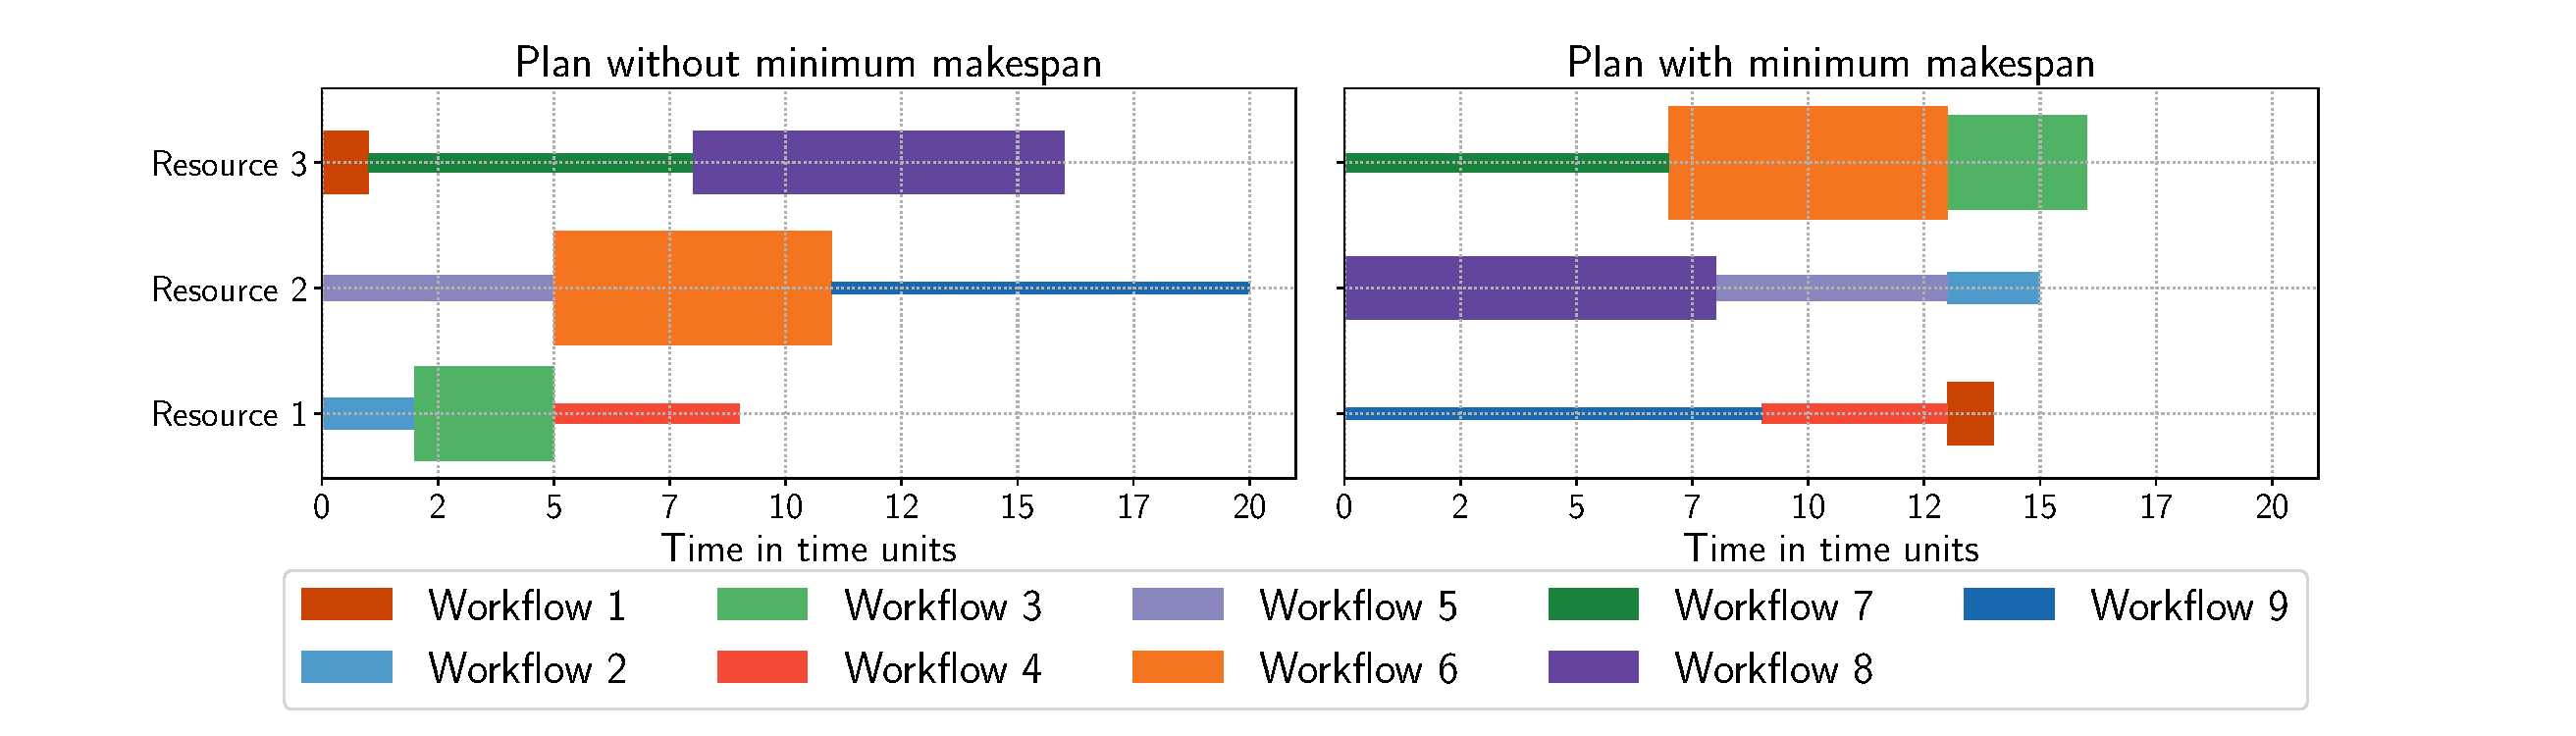
\includegraphics[width=.99\textwidth]{figures/campaign/plan_comp.pdf}
    \caption{Comparison of different campaign execution plans. Based on workflow mapping on resources makespan and resource utilization is different.}\label{fig:example_makespan}
\end{figure*}

We are making a set of assumptions which we do not relax during the initial analysis of a model that calculates the makespan of a campaign.
These are:
\begin{inparaenum}[(1)]
    \item a workflow is an atomic unit and cannot be decomposed;
    \item workflow resource request is sufficient to execute the workflow;
    \item a resource is an aggregate of computing capabilities;
    \item resources are homogeneous;
    \item every workflow of a given campaign can be executed on the given resources;
    \item a random resource selection is based on a uniform distribution;
    \item only one workflow can be executed on a resource at any point in time; and
    \item a workflows can be homogeneous or heterogeneous in space---maximum number of resources they need, and time---the amount of time they are executing.
\end{inparaenum}

We denote a computational campaign as $C = [w_{i}: 1 \leq i \leq N_{C}]$, where $w_{i}$ is a workflow and $N_{C}$ is the total number of workflows, $R = [ r_{j}: 1 \leq j \leq N_{R}]$ is a set of available resources, where $r_{j}$ is a resource and $N_{R}$ is the total number of available resources, and $ M(C,R) = [(w_i, r_j): 1 \leq i \leq N_{C}, r_j \in R] $ is a mapping function of workflows onto resources.
In addition, we denote the execution time of a workflow as $Tx_{w_{i}}$, the makespan of campaign $C$ as $TTX_{C}$, and the makespan of campaign $C$ for a given mapping function $ M $ as $TTX_{C}(M)$.
Assumption~\#3 allows to abstract the resource implementation details, as workflows can be executed on different resources such as HPCs, Clouds, pilots and more. 
Lastly, we will assume homogeneous resources as it simplifies the formalization of the problem.

With a single resource, i.e., $N_{R} = 1$, the workflows of a campaign will be executed sequentially, regardless the execution order or if the workflows are homogeneous or heterogeneous.
As a result the makespan of the campaign is:
\begin{equation}
   TTX_{C} = \sum_{i=1}^{N_{C}}Tx_{w_{i}} 
\end{equation}

With multiple homogeneous resources, i.e., $1 < N_{R} < N_{C}$, the workflows of a campaign can be executed concurrently.
Furthermore, this is semantically equivalent to executing on a single resource large enough to allow concurrent workflow execution, where each workflow executes on a resource partition. 
Because of assumptions~\#5 and~\#7, executing homogeneous or heterogeneous in space workflows has the same makespan.
A random mapping of workflows onto resource will have a makespan:
\begin{equation}
   TTX_{C}(Random) \geq \frac{1}{N_{R}}\sum_{i=1}^{N_{C}} Tx_{w_{i}} 
\end{equation}
Given multiple homogeneous resources, when executing workflows that are heterogeneous in time and that can be homogeneous or heterogeneous in space, the makespan of the campaign for a given mapping function $ M $ is:
\begin{equation}
TTX_{C}(M) = \max_{r_{j}\in R}\Big\{\sum_{w_{i}\in M(C,r_{j})}Tx_{w_{i}}\Big\}
\label{eq:makespan}
\end{equation}

% -------------------------------------------------------------------
\section{Makespan calculating algorithms}
\label{sec:algo}

There is a plethora of methods and algorithms to calculate and optimize the makespan of a workflow~\cite{lu2019review}, including queuing networks~\cite{yao2019throughput,bao2019performance}, domain specific languages~\cite{carothers2017durango,maheshwari2016workflow}, and machine learning~\cite{witt2019predictive,pumma2017runtime}.
From this plethora of selections, we selected to investigate three algorithms, each one representative of a larger family of algorithms.
These are Heterogeneous Earlier Finish Time algorithm (HEFT)~\cite{topcuoglu2002performance}, a genetic algorithm~\cite{page2005algorithm} and a .... algorithm.

% -------------------------------------------------------------------
\subsection{Heterogeneous Earlier Finish Time (HEFT) algorithm}
\label{algo:heft}
List scheduling algorithms represent a general family of heuristic based scheduling algorithms to schedule workflows described as direct acyclic graphs~\cite{dong2006scheduling,list_sched_wiki}. 
These algorithms assign priorities to tasks based on a heuristic and them non-increasingly based on the derived priorities.
Then, this list is traversed and tasks are assigned to resources.
HEFT is a classic example of this type of algorithms~\cite{dong2006scheduling}.

HEFT is an offline scheduling algorithm which calculates the makespan of a workflow on heterogeneous resources, in terms of performance.
HEFT has been implemented as part of the planning capabilities in Pegasus~\cite{deelman2015pegasus} and ASKALON~\cite{fahringer2005askalon} amongst other algorithms.
HEFT has been shown to provide better performance in terms of makespan minimization compared to other mapping algorithms~\cite{topcuoglu2002performance,fahringer2005askalon,canon2008comparative}. 

HEFT makes two important assumptions when used on multiple workflows, i.e., a campaign: 
\begin{inparaenum}[(1)] 
    \item any task in a workflow can be executed on all available resources; and 
    \item all resources are always available.
\end{inparaenum}
HEFT is mainly used to derive an execution plan for workflows, i.e., the execution order and resource placement of the tasks that comprise the workflow.
HEFT uses a matrix to represent execution time of tasks on resources, assigning tasks to the resource that minimizes the finish time of the task, and has complexity proportional to the number of dependencies between tasks and the number of resources offered. 
Because we are interested in campaigns, our HEFT extension will provide an execution plan based on workflows as atomic units instead of tasks.
Furthermore, there has been some initial research to extend HEFT to resources that provide CPU and GPUs~\cite{shetti2013optimization}, as well as a HEFT extension on dynamic resources~\cite{dong2007pfas}. 
Algorithm~\ref{alg:heft} shows HEFT for placing independent heterogeneous workflows on heterogeneous resources.

\begin{algorithm}[ht]
    \caption{Heterogeneous Earliest Finish Time (HEFT) algorithm}
    \label{alg:heft}
    \begin{algorithmic}[1]
        \Procedure{HEFT}{$W$,$R$}\Comment{$W$ and $R$ are a set of workflow and resources respectively}
        \State \texttt{Calculate the computation cost $w_{tx}^{ij}$ of each workflow for all resources}
        \State \texttt{Assign $rank_i = \overline{w_{i}} = \nicefrac{\sum_{j=1}^{|R|}w_{tx}^{ij}}{|R|}$}
        \State \texttt{Sort workflows by non-increasing order of $rank_i$}
        \While{unscheduled workflows}
        \State \texttt{Select the first workflow $\tilde{w}$ from the sorted list}
        \For{$\forall r_{j}$ in $R$}
        \State\texttt{Compute earliest finish time for $\tilde{w}$ on $r_{j}$, $eft_{\tilde{w},r_j}$ }
        \EndFor
        \State \texttt{Assign  $\tilde{w}$ on $r_k$ with $\min{(eft_{\tilde{w},r_j})}$}
        \EndWhile
        \EndProcedure
    \end{algorithmic}
\end{algorithm}

As mentioned above HEFT makes the assumption that all resources are always available and static.
Based on this assumption, HEFT makes the implicit assumption that resources are available based on the times it internally computes.
As a result, it has no external knowledge or representation of when a resource becomes available.
HPC resources may become unavailable for multiple reasons, including but not limited to maintenance, a random failure, executing a workflows over the expected time., etc.
In order to be able to utilize HEFT for dynamic resources, we had to extend Algorithm~\ref{alg:heft} to take as input the time that a resource is initially available.
This input can be represented as a dictionary where the keys are the available resources and the values are the time a resource becomes available.
The extended algorithm is shown in Algorithm~\ref{alg:ext_heft}.
Although the extension may be small, it is crucial to allow to reuse HEFT based on the state of the execution at a given point in time.

\begin{algorithm}[ht]
    \caption{Extended Heterogeneous Earliest Finish Time (EHEFT) algorithm}
    \label{alg:ext_heft}
    \begin{algorithmic}[1]
        \Procedure{EHEFT}{$W$, $R$, $T$}\Comment{$W$ and $R$ are a set of workflow and resources respectively. $T$ is a dictionary of when a resource becomes available.}
        \State \texttt{Calculate the computation cost $w_{tx}^{ij}$ of each workflow for all resources}
        \State \texttt{Assign $rank_i = \overline{w_{i}} = \nicefrac{\sum_{j=1}^{|R|}w_{tx}^{ij}}{|R|}$}
        \State \texttt{Sort workflows by non-increasing order of $rank_i$}
        \While{unscheduled workflows}
        \State \texttt{Select the first workflow $\tilde{w}$ from the sorted list}
        \For{$\forall r_{j}$ in $R$}
        \State\texttt{Compute earliest finish time for $\tilde{w}$ on $r_{j}$ based on $T(r_j)$, $eft_{\tilde{w},r_j}$ }
        \EndFor
        \State \texttt{Assign  $\tilde{w}$ on $r_k$ with $\min{(eft_{\tilde{w},r_j})}$}
        \EndWhile
        \EndProcedure
    \end{algorithmic}
\end{algorithm}

% -------------------------------------------------------------------
\subsection{Genetic algorithm}
\label{algo:gen}
Genetic algorithms are represent another family of algorithms that are been used to minimize the makespan of an execution~\cite{dong2006scheduling}.
Genetic algorithms are evolving to the final answer as they iterate and improve possible answers.
In general, genetic algorithms are working based on the following procedure:
\begin{inparaenum}[(i)]
    \item create an initial population, where the population is a set of chromosomes. 
          Chromosomes, in the context of planning the execution workflows on resources, is a potential placement of workflows on resources;
    \item evaluate the chromosomes based on a fitness value, which represents the makespan on the campaign;
    \item reproduce by selecting chromosomes, either randomly or based on their fitness value, and generate a new set of chromosomes (called children);
    \item mutate randomly, where randomly selected workflows from a random chromosome are reassigned to resources; and
    \item re-evaluate chromosomes in the population to check convergence.
\end{inparaenum}

The selected genetic algorithm~\cite{page2005algorithm} is developed to support the placement of independent task on heterogeneous resources.
It assumes that all tasks can be executed on all available resources, are independent and indivisible.
These assumptions are in accordance with the assumptions made for workflows in a campaign.
As a result, this algorithm can be extended to support scientific campaigns.
The pseudocode of this algorithm is shown in Algorithm~\ref{alg:gen_algo}.

\begin{algorithm}[ht]
    \caption{Genetic Algorithm}
    \label{alg:gen_algo}
    \begin{algorithmic}[1]
        \Procedure{GA}{$W$, $R$, $T$}\Comment{$W$ and $R$ are a set of workflow and resources respectively. $T$ is a dictionary of when a resource becomes available.}
        \State \texttt{Initaliaze population}
        \While{Conergence Criteria not met and \#Gen $<$ Total\_Generations}
        \State{Selection}
        \State{Reproduce}
        \State{Randomly mutate}
        \State{Balance}
        \EndWhile
        \EndProcedure
    \end{algorithmic}
\end{algorithm}

The chromosomes of the initial population are constructed semi-random.
Specifically, a specific percentage of the workflows are assigned randomly to resources, where the assignment is drawn by uniform distribution.
The rest of the workflows are assigned based on an earlier finish time (EFT) heuristic, similar to the one used by HEFT.
The population size is relatively small to 20 chromosomes, i.e., potential plans, called micro-GA.
Micro-GA reduces the computational load of the genetic algorithm, while it does not significantly impact the final result~\cite{zomaya2001observations}.

Selection of the chromosomes to reproduce is based on a fitness function, which calculates the relative distance from a theoretical optimal processing time.
Each chromosome is assigned a fitness value, which then defines the probability of a chromosome to be selected.
Reproduction uses cyclic rotation to generate the new population members.
Mutation randomly selects an individual from the population and randomly swaps workflows.
Finally, a rebalancing heuristic tries to rebalance and create fitter individuals in the population.

We extend this algorithm in the population initialization to support replanning..
The initialization method takes into account the times resources will be available during for the EFT heuristic.
Another point of extension would be the fitness function.
However, the fitness function of the selected algorithm~\cite{page2005algorithm} already takes into account the previous load of a resource, which is the time a resource is available.

% -------------------------------------------------------------------
\subsection{Largest to fastest algorithm}
\label{algo:l2ff}
The last algorithm places workflows based on the rule largest workflows to fastest resource~\cite{balasubramanian2019programming}.
This algorithm sorts the workflows based on the number of operations and resources based on their performance.
Then it places workflows on resources in a round robin fashion.
Algorithm~\ref{alg:l2ff} show the pseudocode for this algorithm.

\begin{algorithm}[ht]
    \caption{Longest to Fastest First (L2FF)}
    \label{alg:l2ff}
    \begin{algorithmic}[1]
        \Procedure{l2ff}{$W$, $R$}\Comment{$W$ and $R$ are a set of workflow and resources respectively.}
        \State \texttt{$W_{sorted}=sort(W)$} 
        \State \texttt{$R_{sorted}=sort(R)$}
        \For{$w$ in $W_{sorted}$}
        \State{Assign $w$ to $r_{k}$ where $k=w_{idx} \mod N_{R}$}
        \EndFor
        \EndProcedure
    \end{algorithmic}
\end{algorithm}

This algorithm does not specify in any way when resources are either becoming or are available.
As a consequence, there is no need to extend it when dynamic resources are used, as long as the resource performance is updated accordingly.

% -------------------------------------------------------------------
\section{Makespan algorithm performance comparison}
\label{sec:algo_perf_comp}

We executed two experiments in order to analyze the performance of the selected planners in terms of the makespan they produce.
In addition to these two experiments, we also executed an experiment to measure the time each planner took to provide a plan.
These sets of experiments allows us to a methodology to compare planning algorithms and decide which algorithm is more suited based on a campaign's computation requirements, i.e. workflow size and resource performance/availability.

\subsection{Experiment 1: Measuring  makespan on static resources}

- Analysis of homogeneous/homogeneous cases:

\begin{figure*}[ht!]
    \centering
    \begin{subfigure}[b]{0.45\textwidth}
        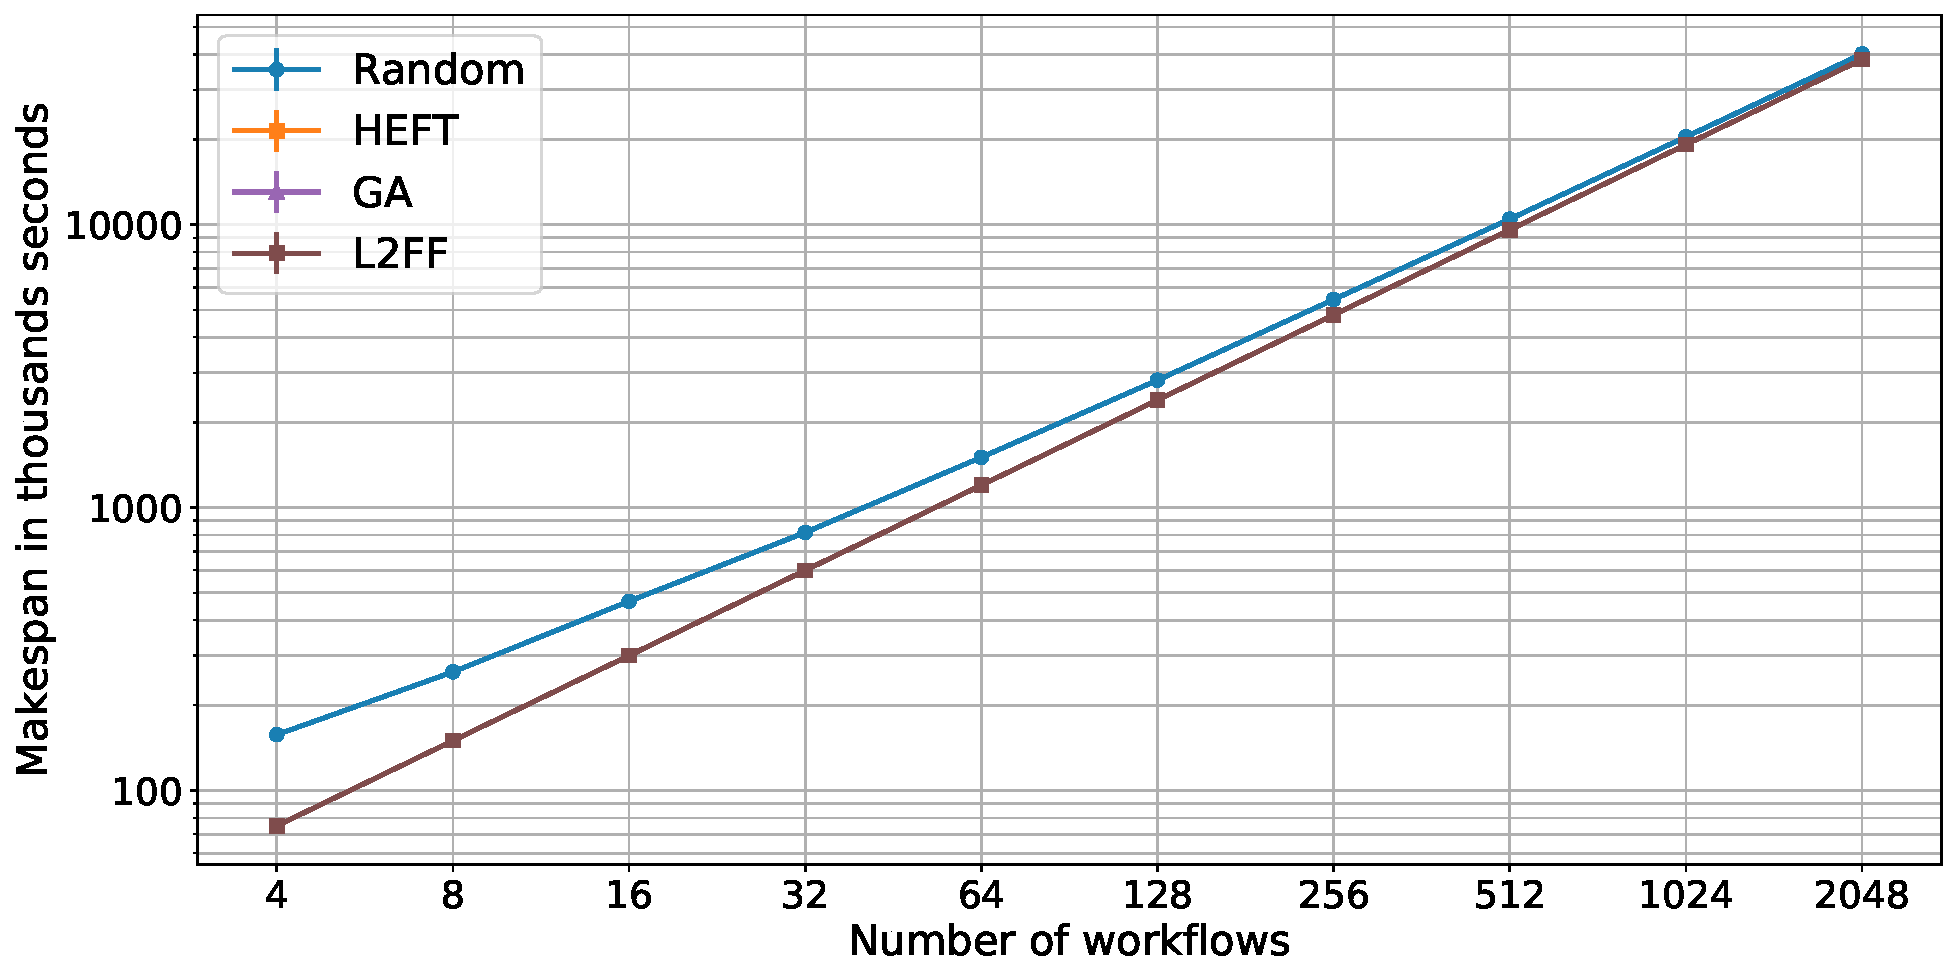
\includegraphics[width=.95\textwidth]{figures/campaign/StHomoCampaigns_4StHomoResources.pdf}
        \caption{}
        \label{fig:StHomoCampaigns_4StHomoResources}
    \end{subfigure}%
    ~ 
    \begin{subfigure}[b]{0.45\textwidth}
        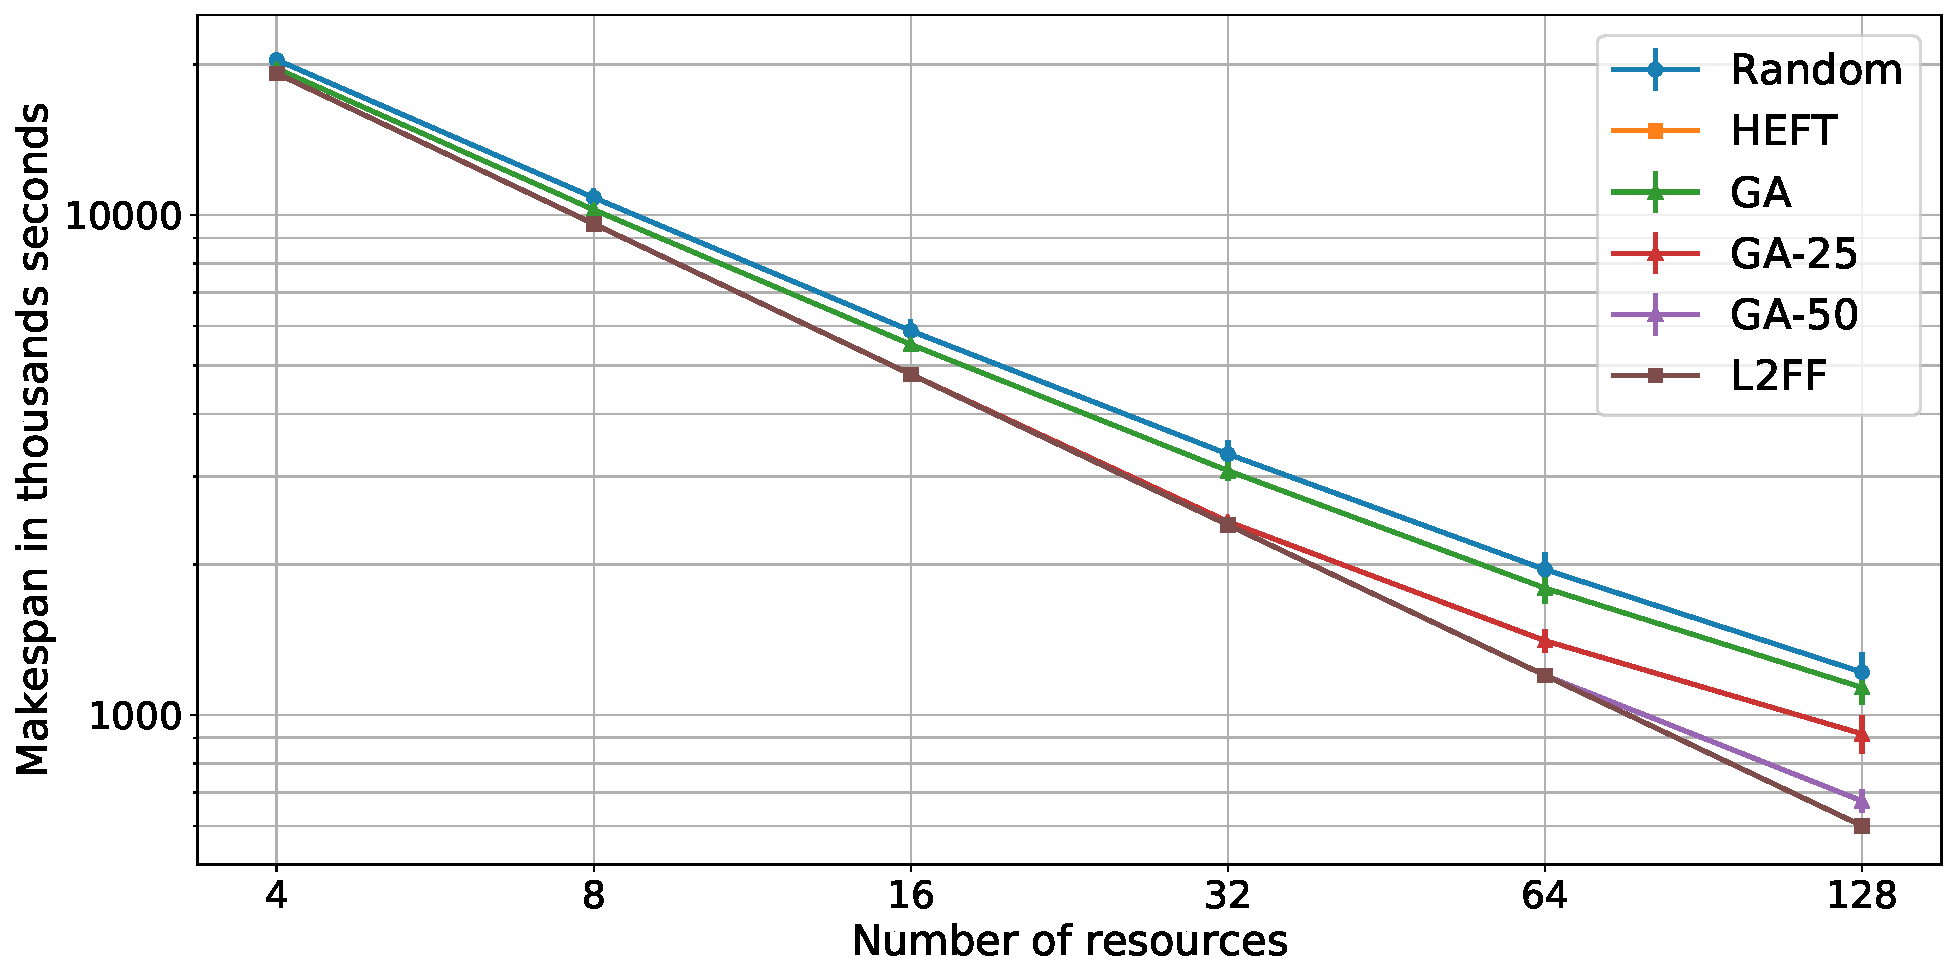
\includegraphics[width=\linewidth]{figures/campaign/StHomoResources_StHomoCampaigns.pdf}
        \caption{}
        \label{fig:StHomoResources_StHomoCampaigns}
    \end{subfigure}
    \caption{~\ref{fig:StHomoCampaigns_4StHomoResources} Makespan of increasing number of homogeneous worklfows on homogeneous resources.
    ~\ref{fig:StHomoResources_StHomoCampaigns} Makespan of homogeneous campaign on different number of homogeneous resources.}
    \label{fig:dyn_homog_analysis}
\end{figure*}



\begin{figure*}[ht!]
    \centering
    \begin{subfigure}[b]{0.45\textwidth}
        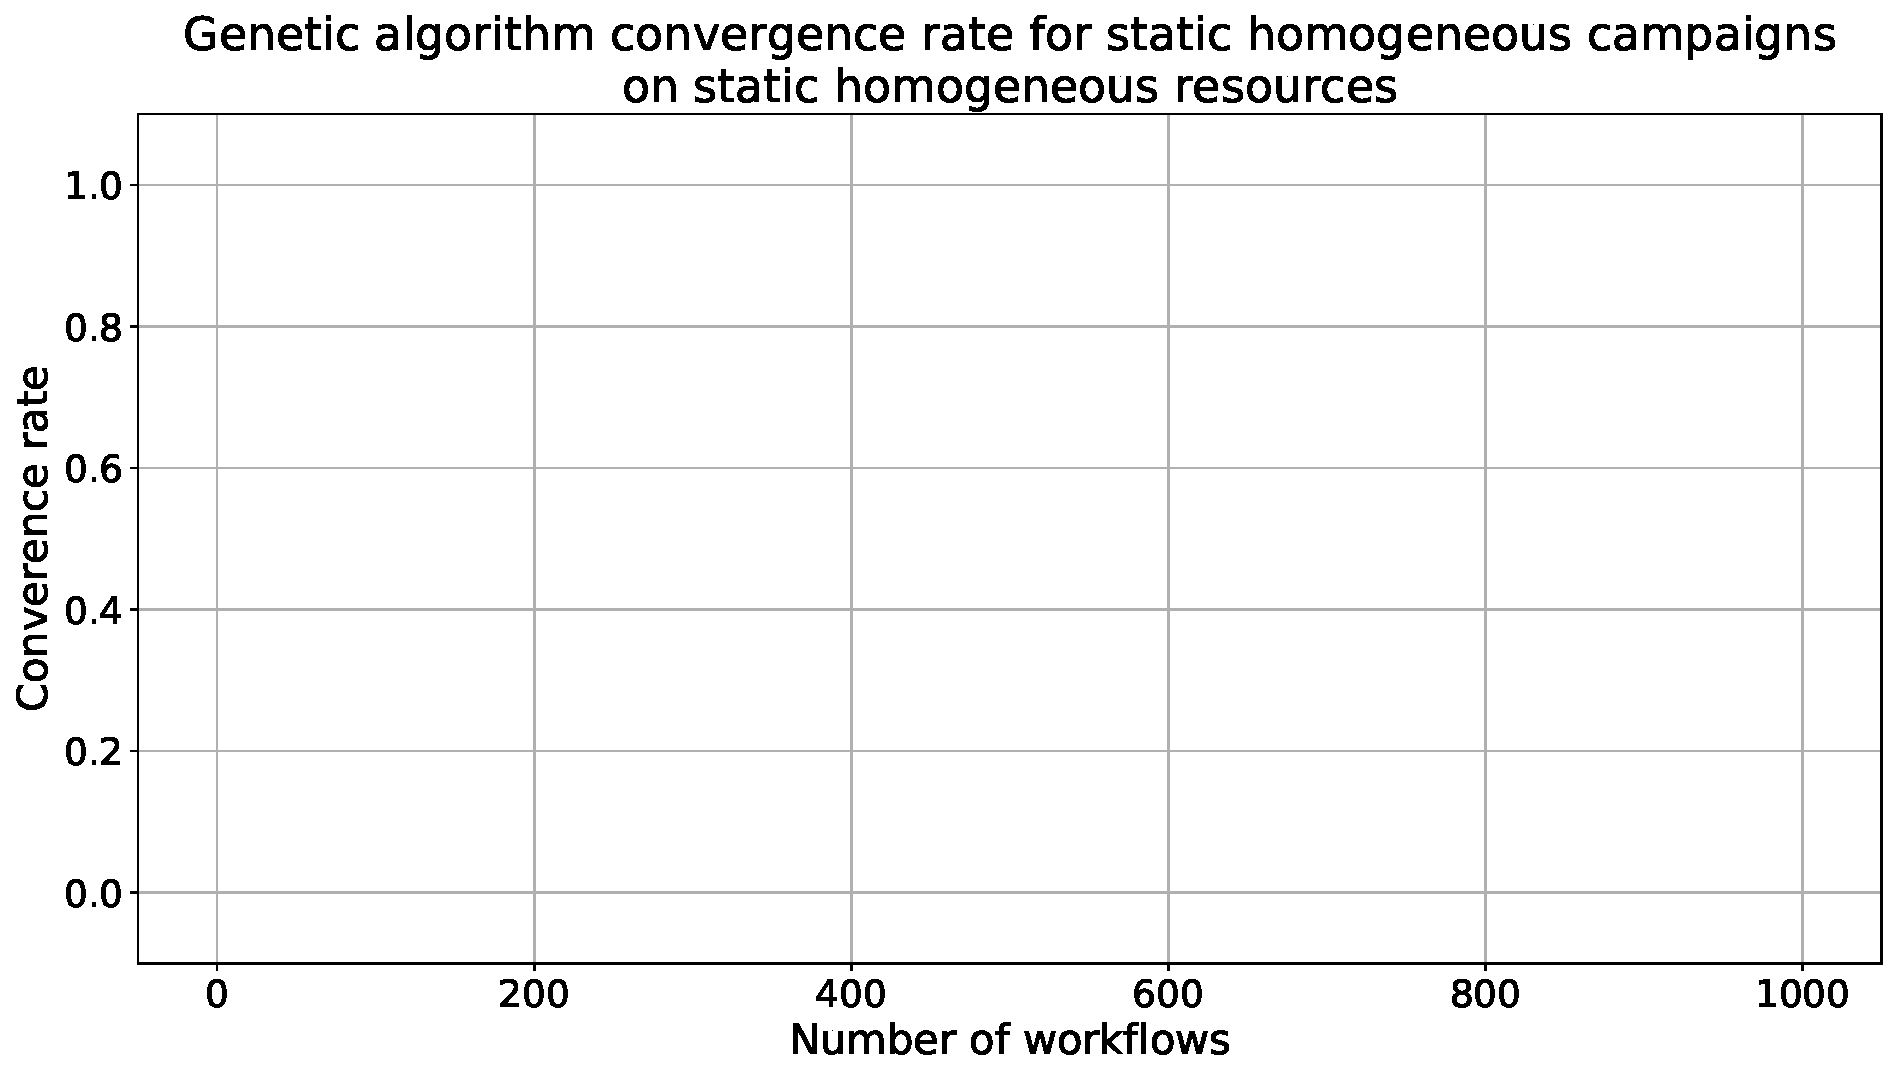
\includegraphics[width=.95\textwidth]{figures/campaign/GAconv_StHomoCampaigns_4StHomoResources.pdf}
        \caption{}
        \label{fig:ga_conv1}
    \end{subfigure}%
    ~ 
    \begin{subfigure}[b]{0.45\textwidth}
        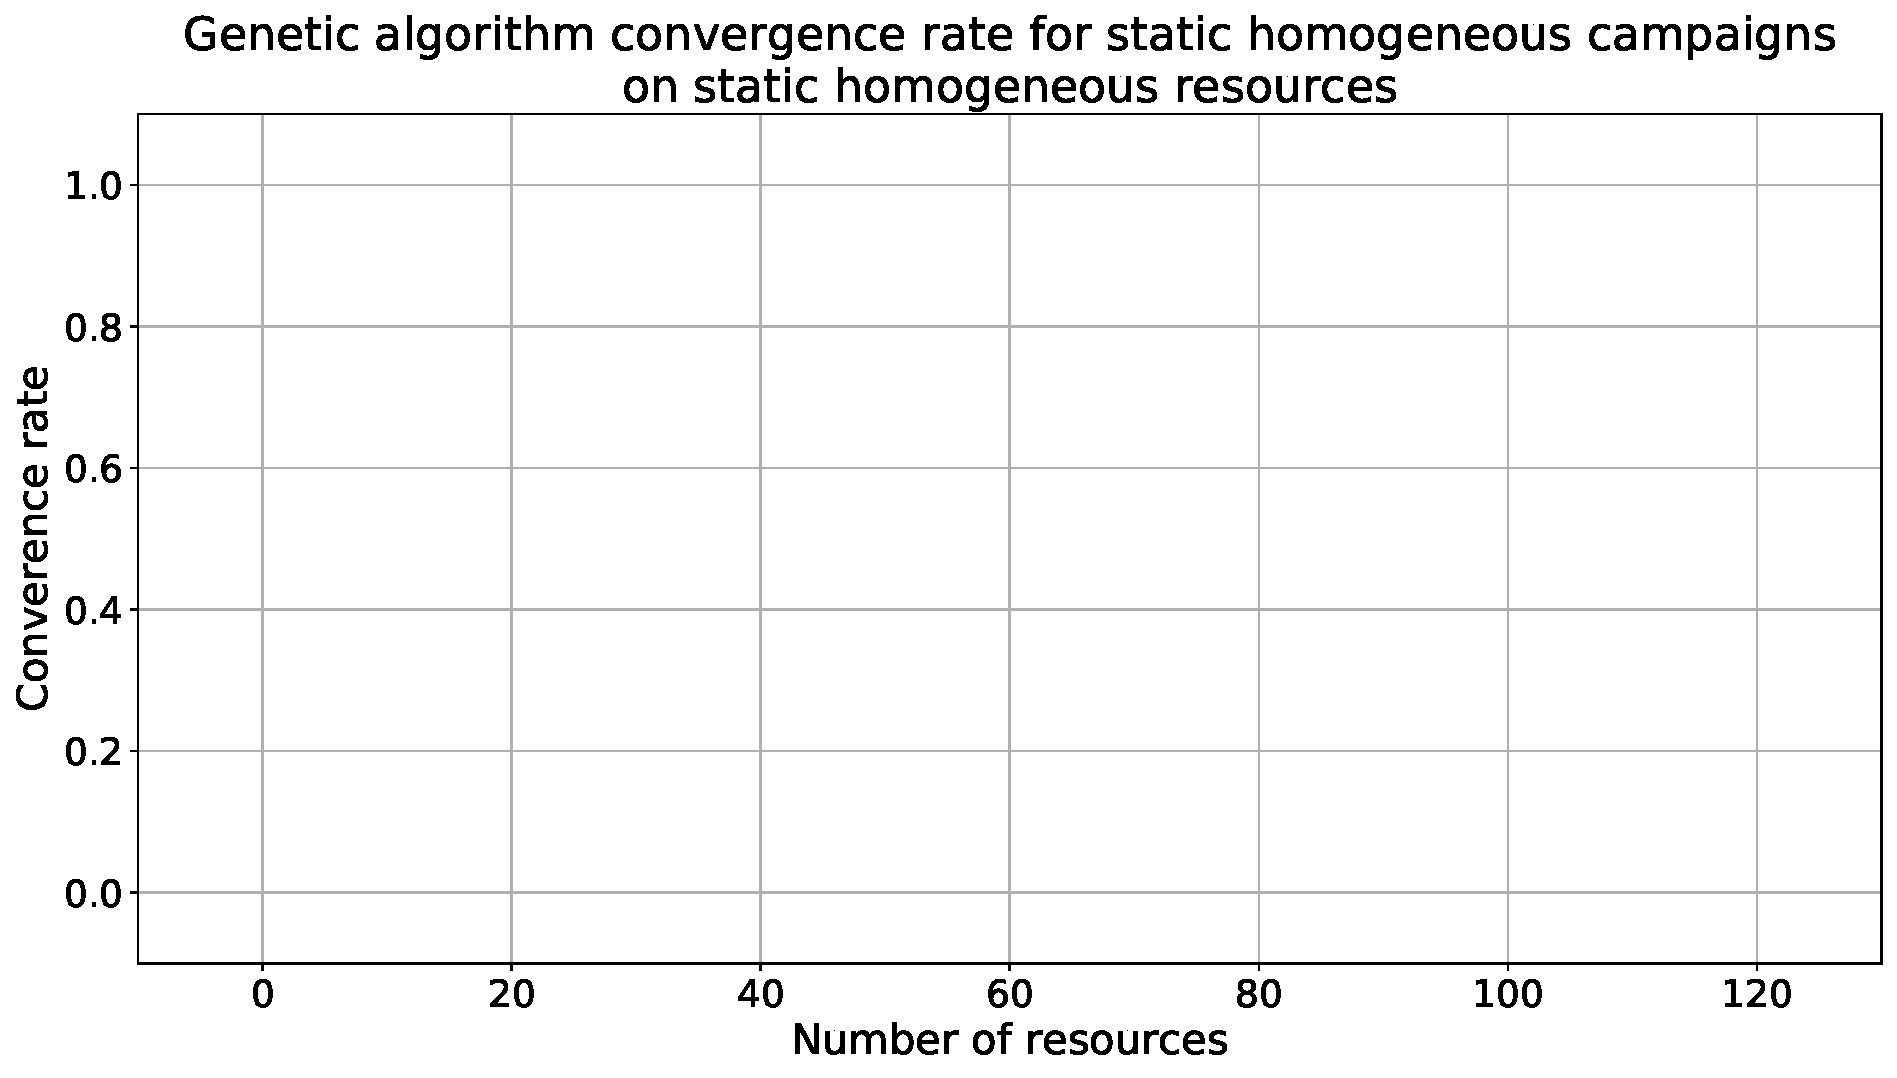
\includegraphics[width=\linewidth]{figures/campaign/GAconv_StHomoResources_StHomoCampaigns.pdf}
        \caption{}
        \label{fig:ga_conv2}
    \end{subfigure}
    \caption{Convergence rate of Genetic algorithm for homogeneous campaigns on static homogeneous resources based on random initialization percentage: ~\ref{fig:ga_conv1}) Different campaign sizes on 4 resources;~\ref{fig:ga_conv2}) Campaign with 1024 workflows and different number of resources.}
    \label{fig:conv_rate}
\end{figure*}

- Analysis of heterogeneous/heterogeneous cases:

\begin{figure*}[ht!]
    \centering
    \begin{subfigure}[b]{0.45\textwidth}
        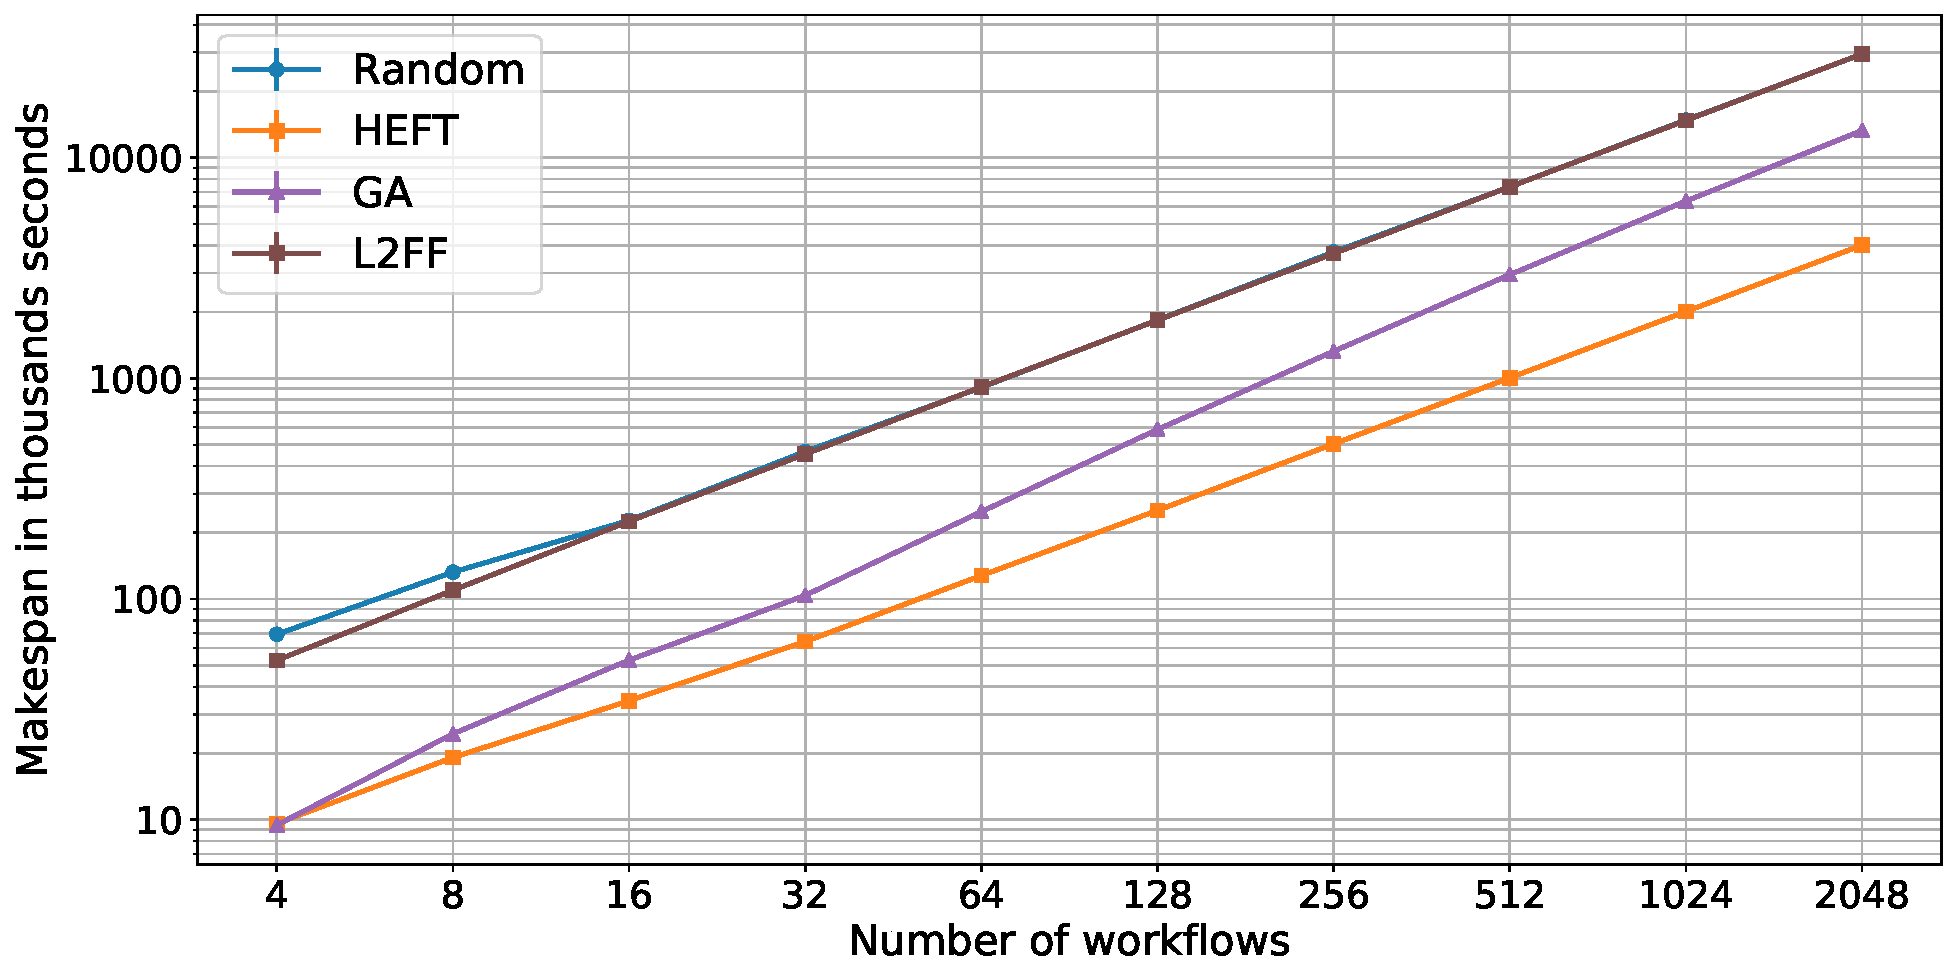
\includegraphics[width=.95\textwidth]{figures/campaign/StHeteroCampaigns_4StHeteroResources.pdf}
        \caption{}
        \label{fig:StHeteroCampaigns_4StHeteroResources}
    \end{subfigure}%
    ~ 
    \begin{subfigure}[b]{0.45\textwidth}
        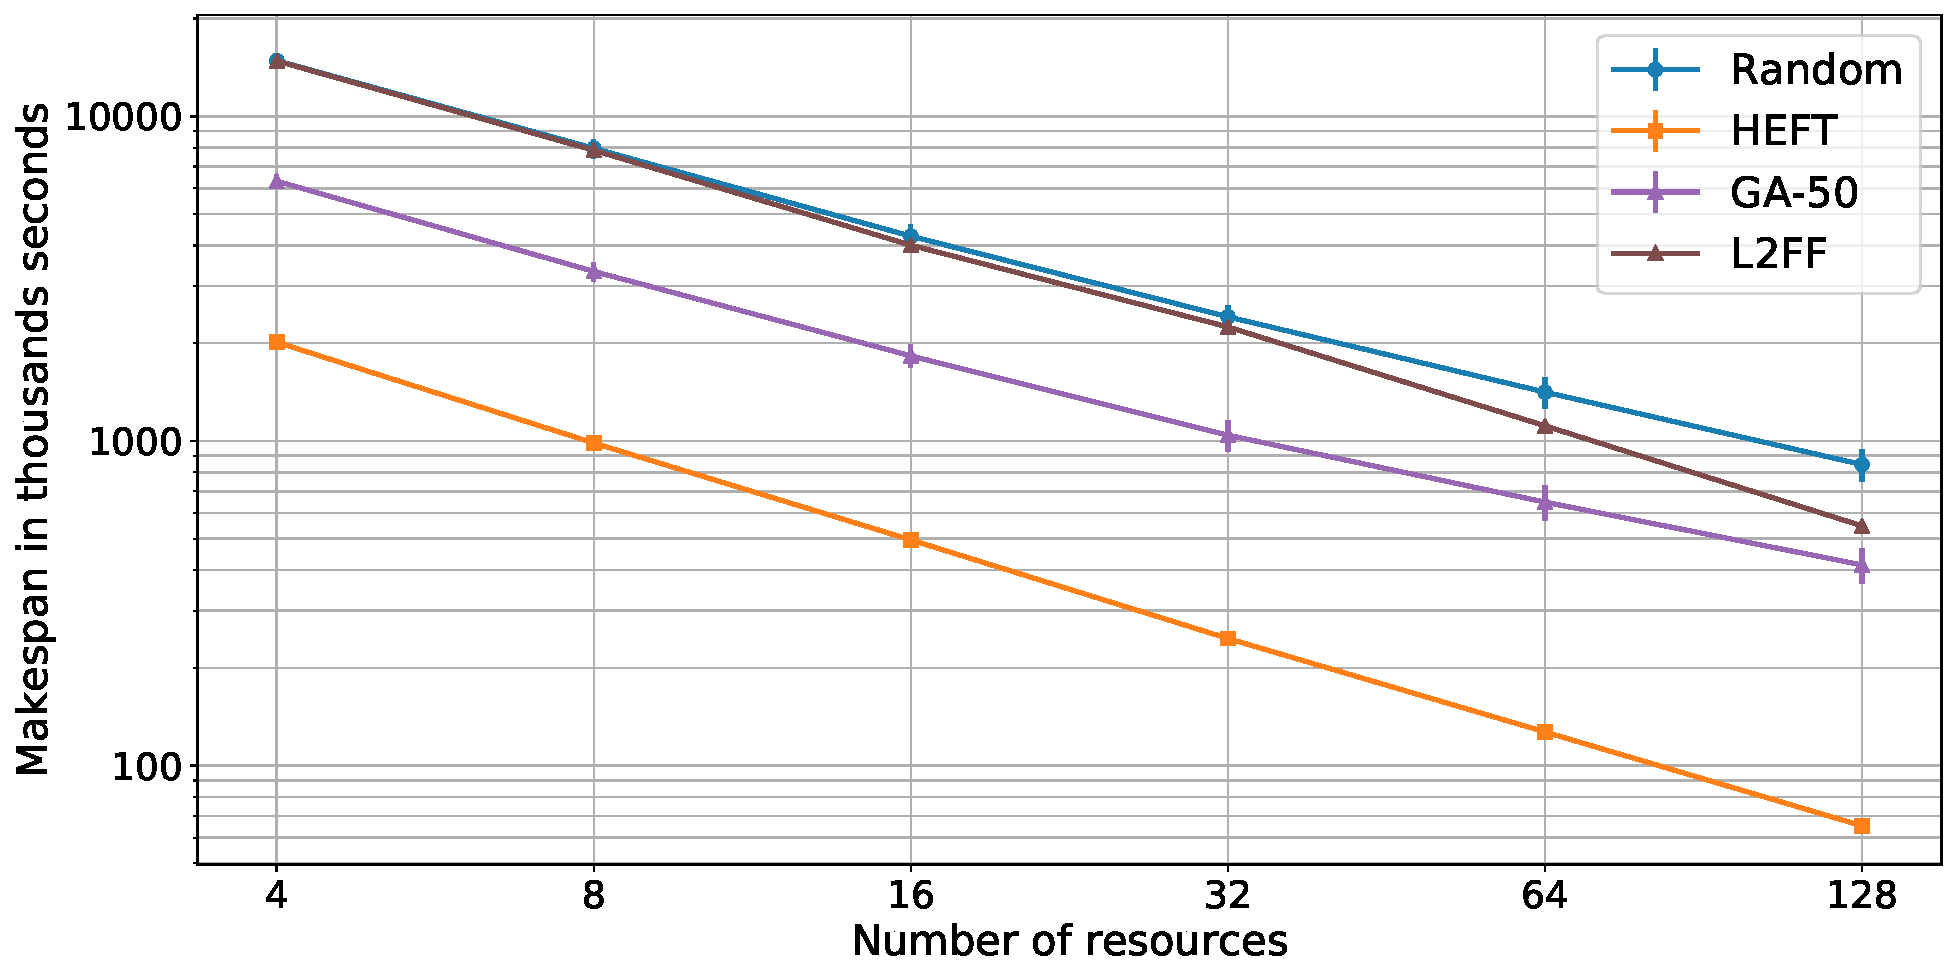
\includegraphics[width=\linewidth]{figures/campaign/StHeteroResources_StHeteroCampaigns.pdf}
        \caption{}
        \label{fig:StHeteroResources_StHeteroCampaigns}
    \end{subfigure}
    \caption{~\ref{fig:StHeteroCampaigns_4StHeteroResources}) Makespan of increasing number of heterogeneous worklfows on heterogeneous resources;
        ~\ref{fig:StHeteroResources_StHeteroCampaigns}) Makespan of heterogeneous campaign on different number of heterogeneous resources..}
    \label{fig:heter_analysis}
\end{figure*}

Generally on Static resources, HEFT provides consistently the best makespan compared to the other algorithms.
This is because: 1) its deterministic behavior, as it produce always the same plan for the same workflows and resources; and 2) its knowledge of when a resource is available.
The genetic algorithm provides worse makespan compared to HEFT mainly because of the randomness introduced during the population initialization.

\subsection{Experiment 2: Measuring makespan on dynamic resources}

\subsubsection{No replanning}

- Analysis of homogeneous/homogeneous cases: Resource dynamism is drawn by a normal distribution.

Since there is no replanning, we just calculate the final makespan based on the plan that was offered initially.
 I expect that HEFT will be better than other planners, with the genetic and the L2FF being very close to random.
\begin{figure*}[ht!]
    \centering
    \begin{subfigure}[b]{0.45\textwidth}
        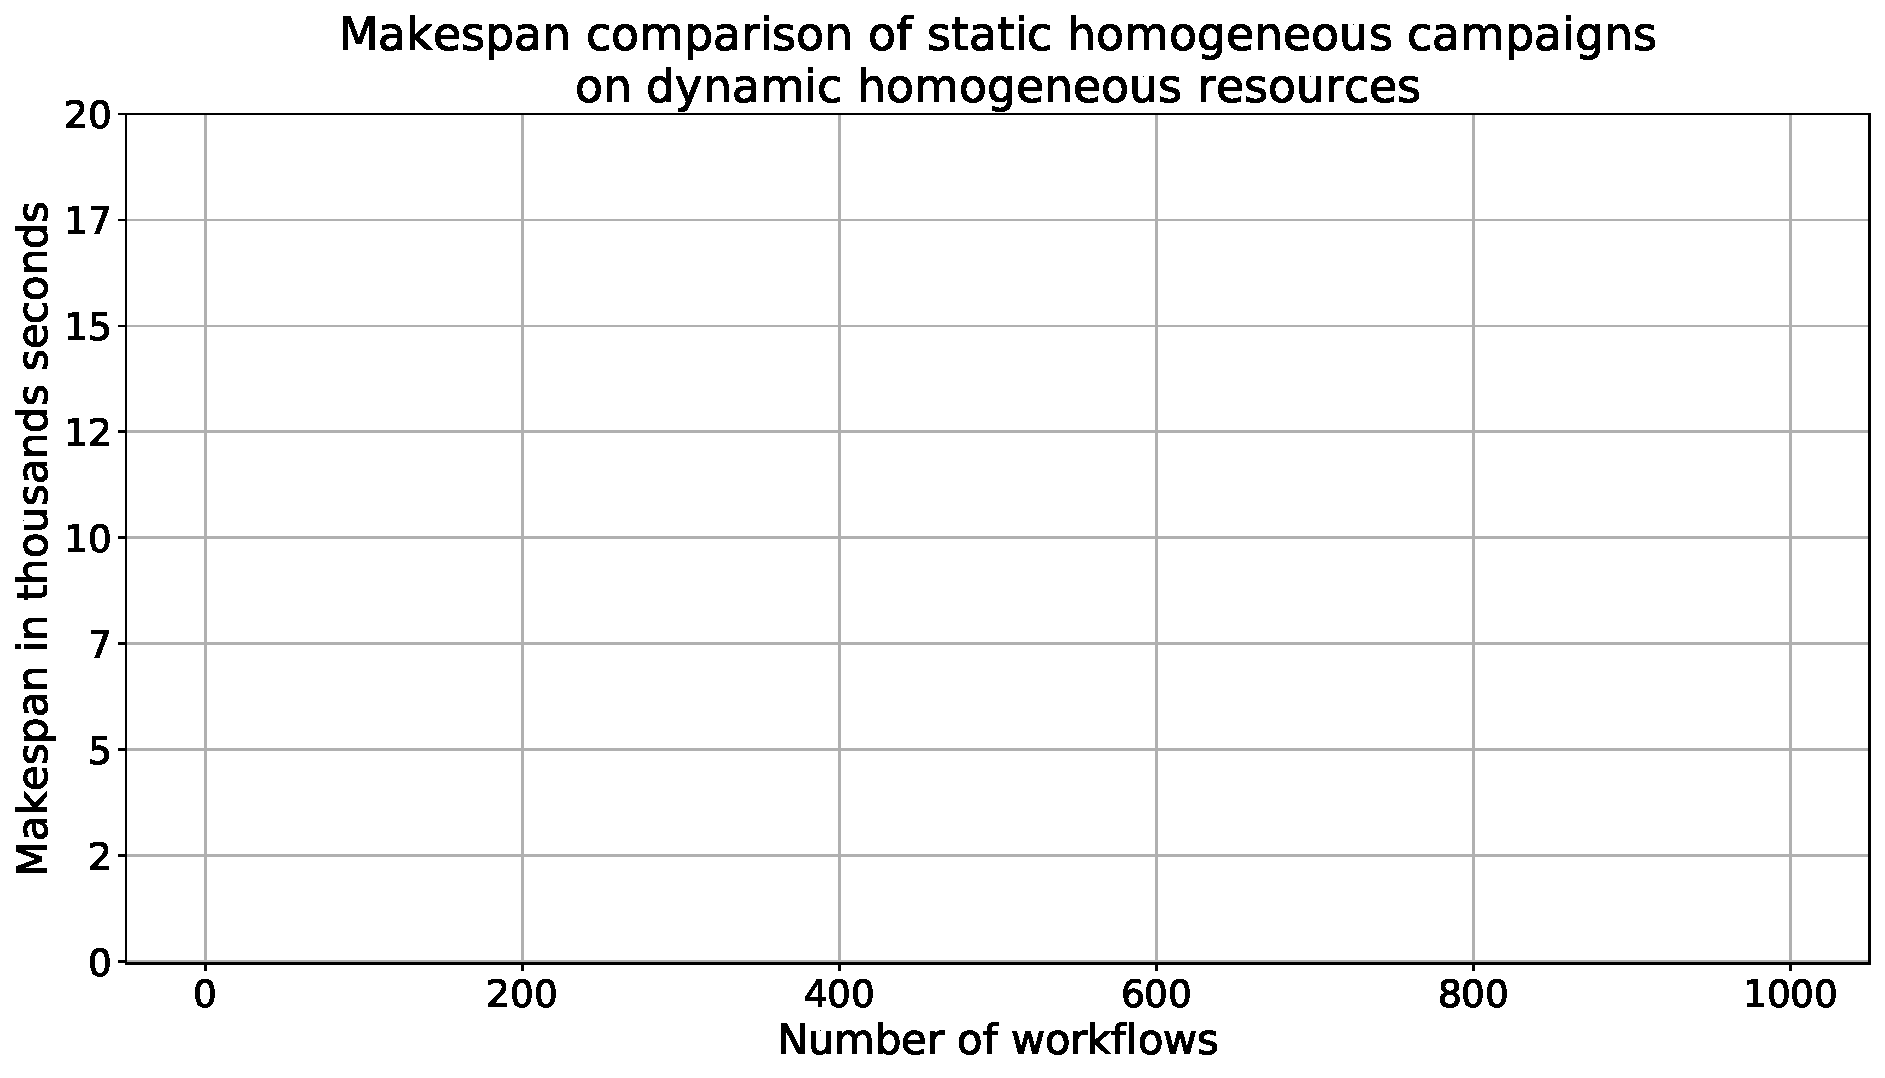
\includegraphics[width=.95\textwidth]{figures/campaign/StHomoCampaigns_4DyHomoResources.pdf}
        \caption{}
        \label{fig:StHomoCampaigns_4DyHomoResources}
    \end{subfigure}%
    ~ 
    \begin{subfigure}[b]{0.45\textwidth}
        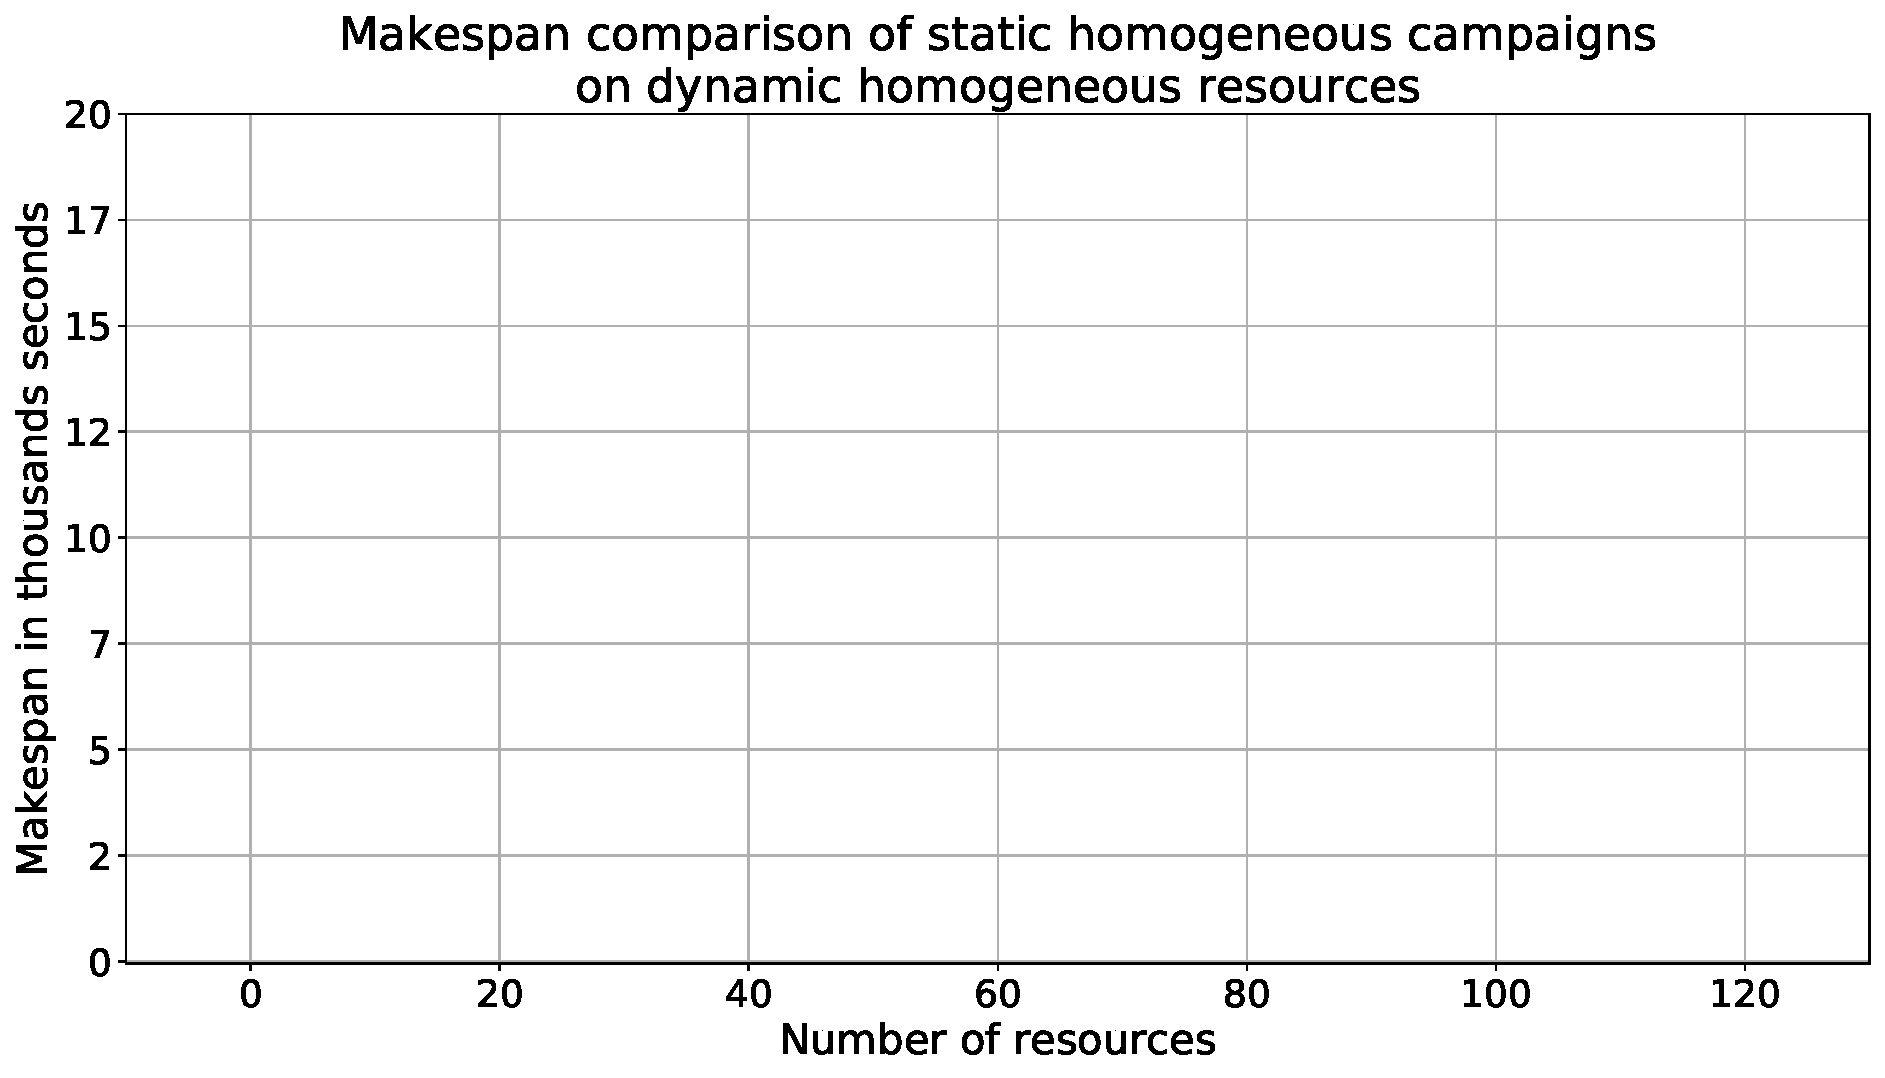
\includegraphics[width=\linewidth]{figures/campaign/DyHomoResources_StHomoCampaigns.pdf}
        \caption{}
        \label{fig:DyHomoResources_StHomoCampaigns}
    \end{subfigure}
    \caption{~\ref{fig:StHomoCampaigns_4DyHomoResources} Makespan of increasing number of homogeneous workflows on homogeneous resources;
        ~\ref{fig:DyHomoResources_StHomoCampaigns} Makespan of homogeneous campaign on different number of homogeneous resources.}
    \label{fig:no_replan_homog_analysis}
\end{figure*}


- Analysis of heterogeneous/heterogeneous cases:
I do not expect significant differences between planners.
I think that the final makespan will be similar for all planners and the will not be distinguishable within error bars.
\begin{figure*}[ht!]
    \centering
    \begin{subfigure}[b]{0.45\textwidth}
        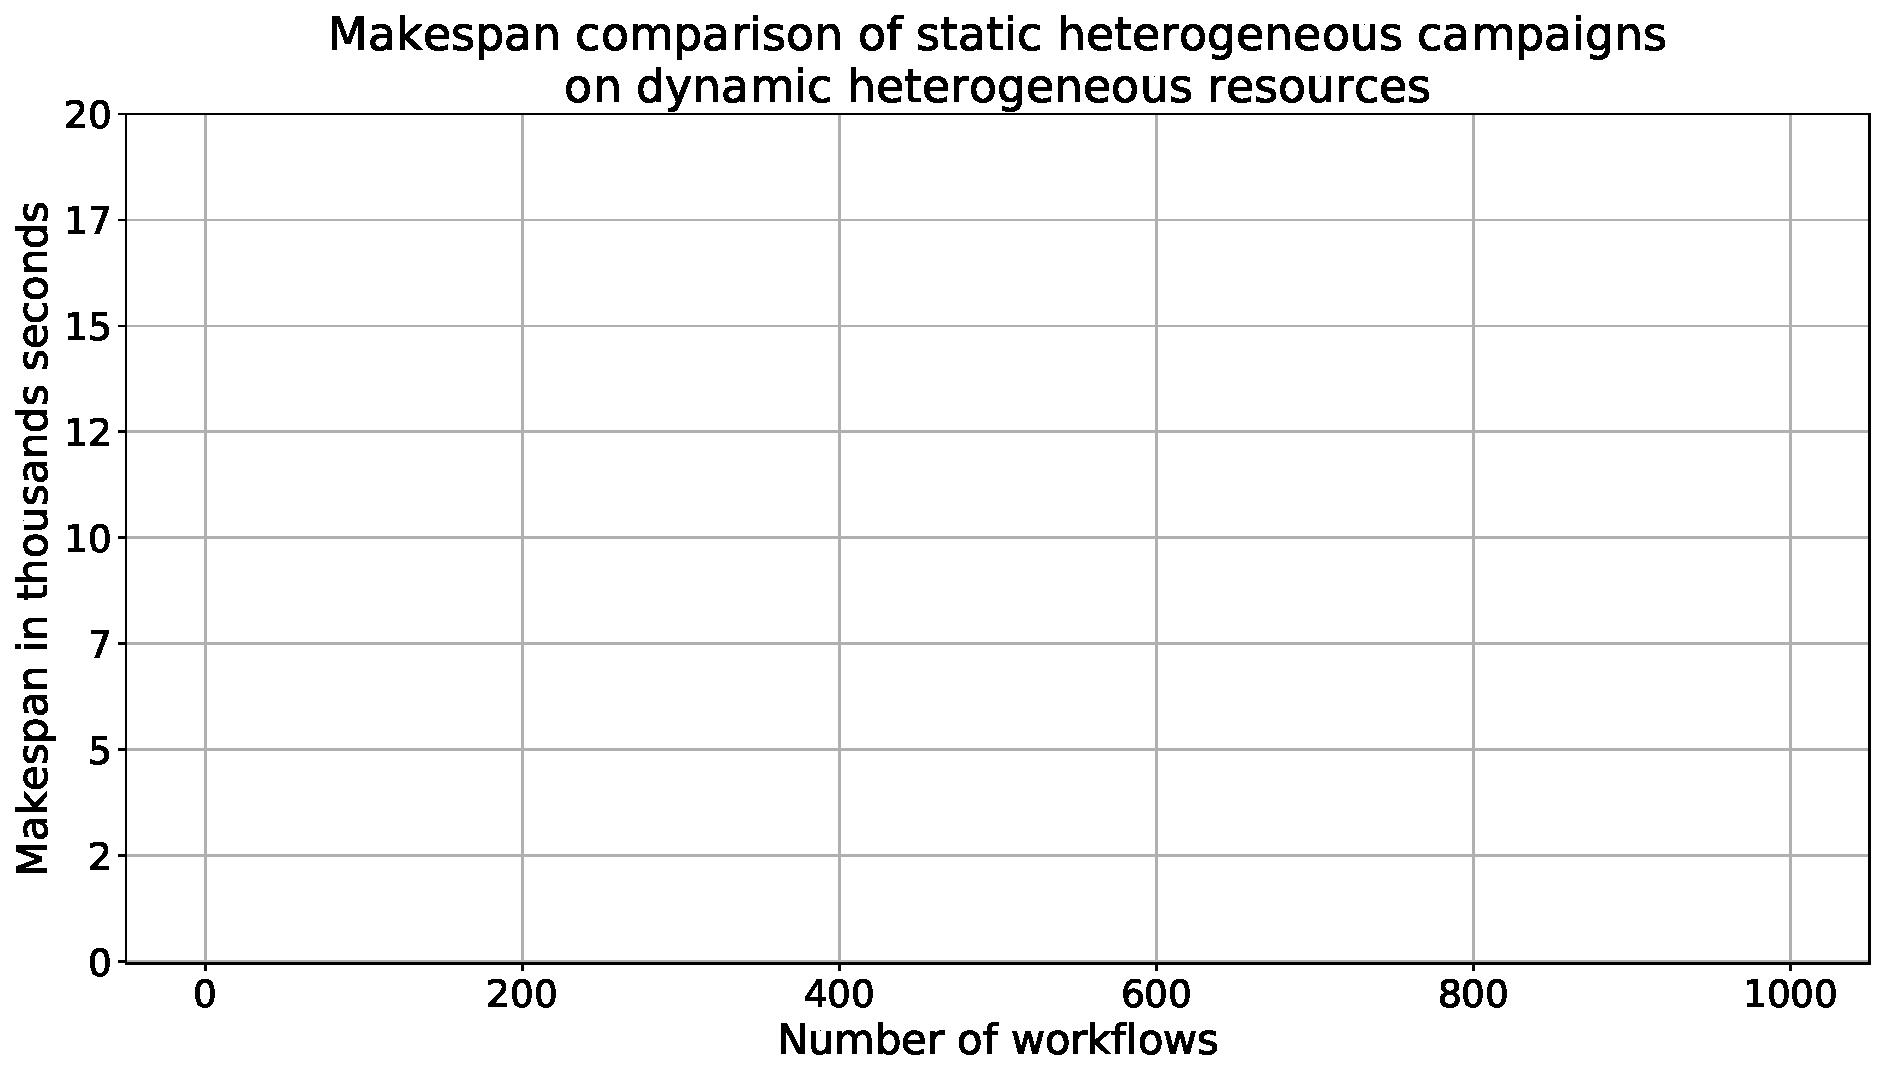
\includegraphics[width=.95\textwidth]{figures/campaign/StHeteroCampaigns_4DyHeteroResources.pdf}
        \caption{}
        \label{fig:StHeteroCampaigns_4DyHeteroResources}
    \end{subfigure}%
    ~ 
    \begin{subfigure}[b]{0.45\textwidth}
        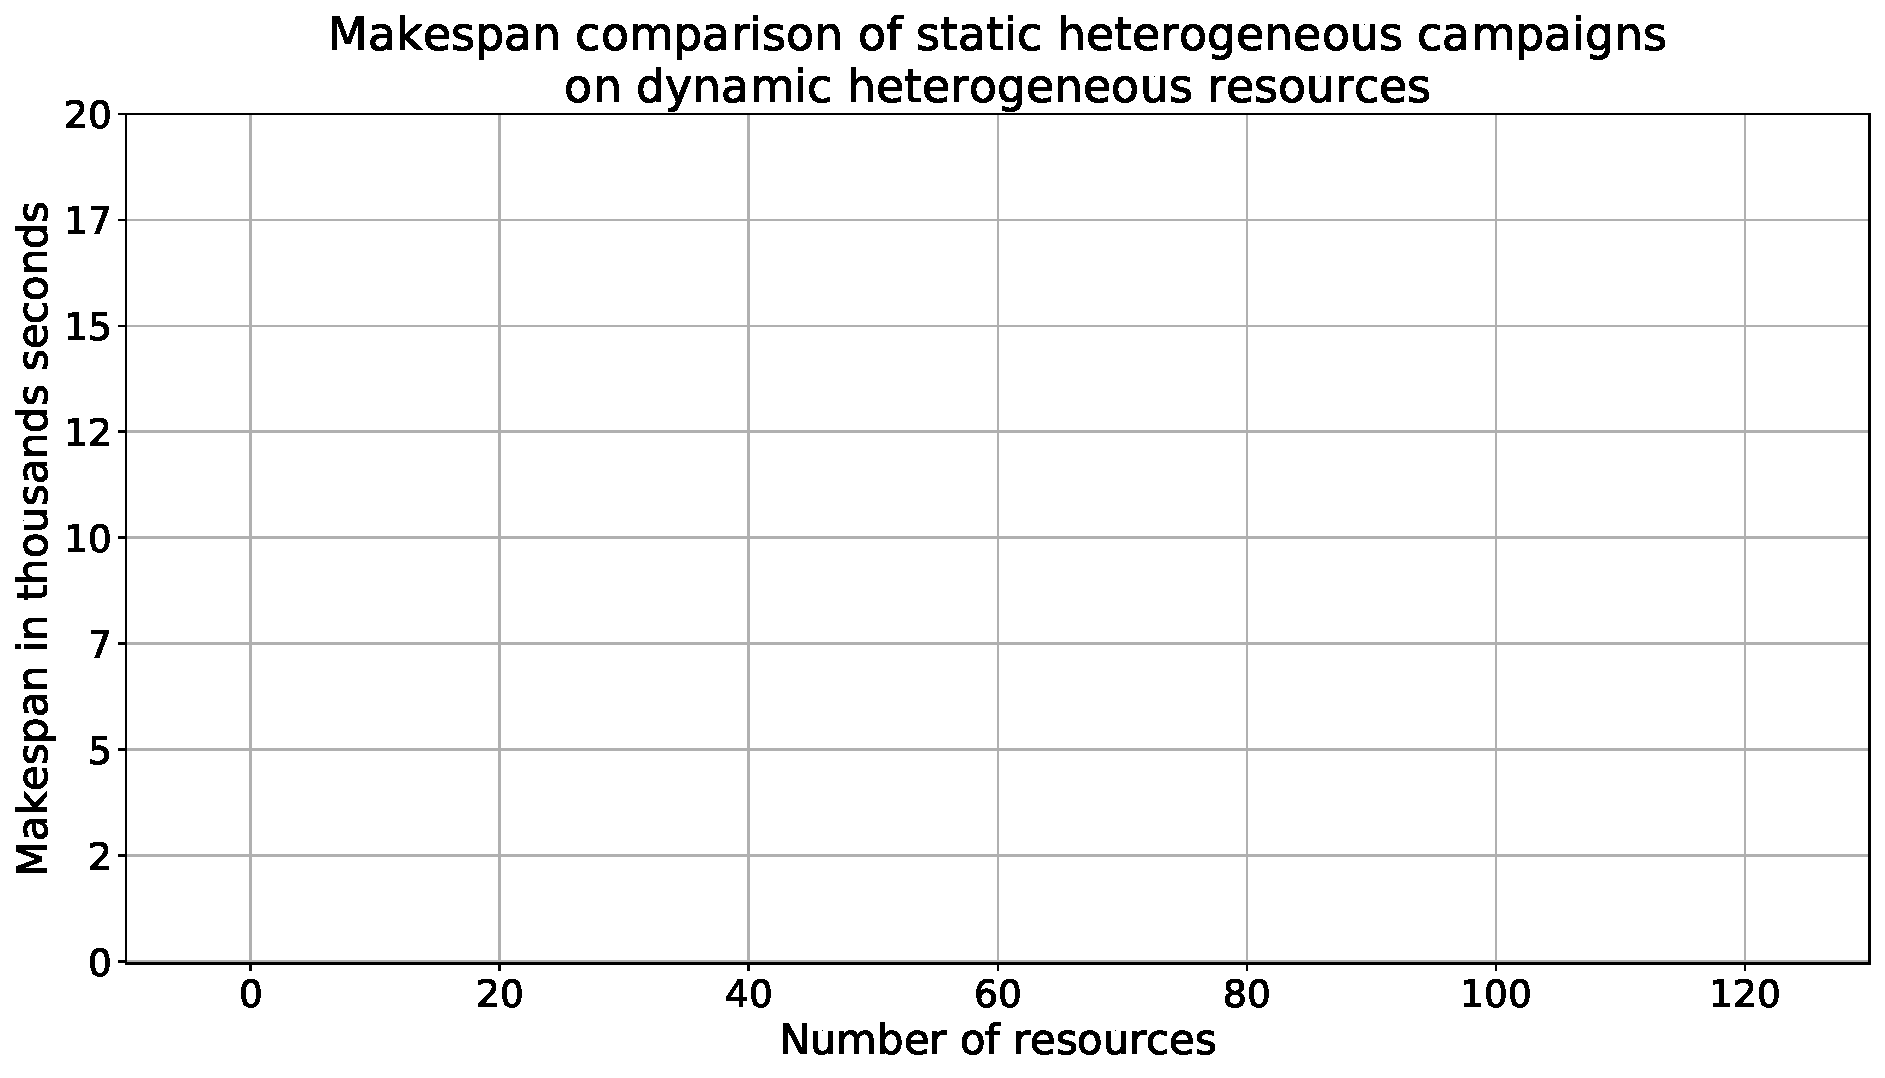
\includegraphics[width=\linewidth]{figures/campaign/DyHeteroResources_StHeteroCampaigns.pdf}
        \caption{}
        \label{fig:DyHeteroResources_StHeteroCampaigns}
    \end{subfigure}
    \caption{~\ref{fig:StHeteroCampaigns_4DyHeteroResources} Makespan of increasing number of homogeneous workflows on homogeneous resources;
    ~\ref{fig:DyHeteroResources_StHeteroCampaigns} Makespan of homogeneous campaign on different number of homogeneous resources.}
    \label{fig:no_replan_hetero_analysis}
\end{figure*}

\subsubsection{Replanning}

Replanning will allow for adjustments of the plan during runtime.
In this case I expect HEFT to provide the better makespan, but I think it is going to be marginally better than the genetic algorithm. 
L2FF will provide a makespan that fluctuates significantly between different cases.
Finally, the random planner will show erratic behavior, depending on the run.

\begin{figure*}[ht!]
    \centering
    \begin{subfigure}[b]{0.45\textwidth}
        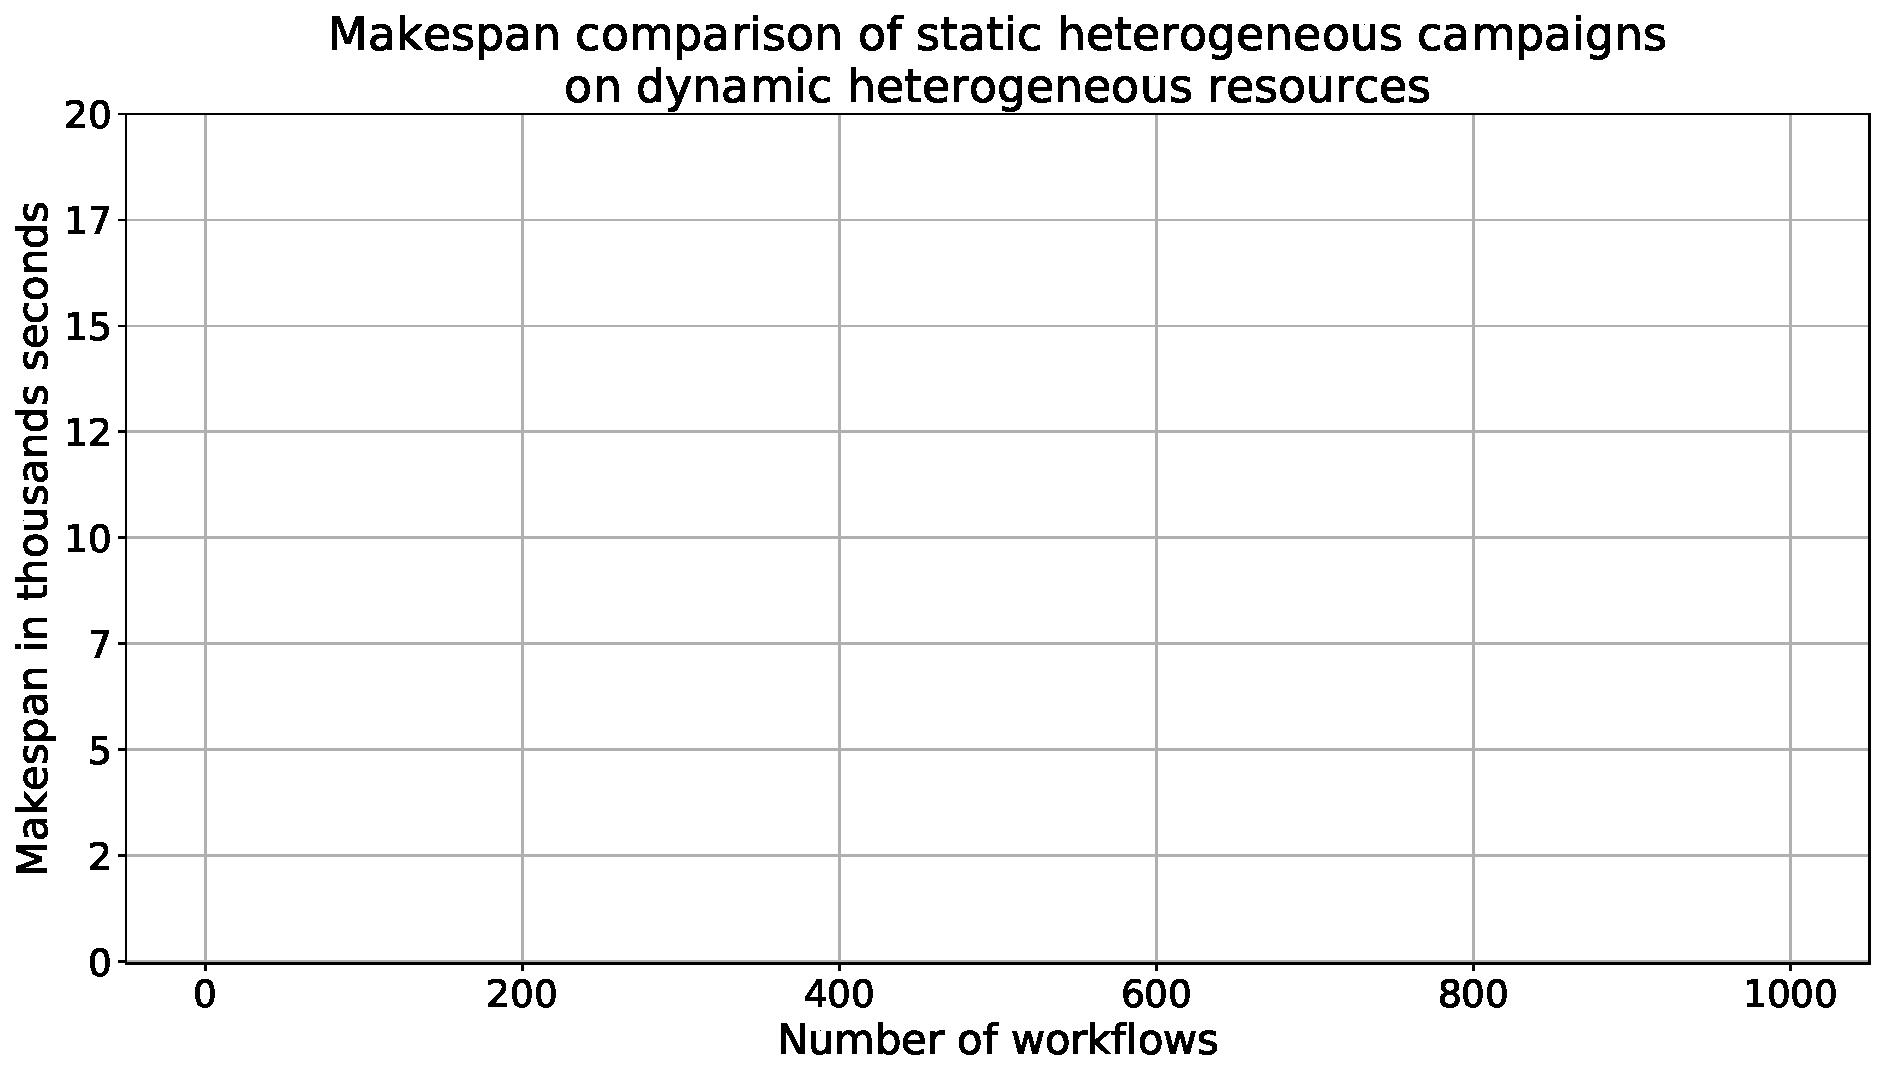
\includegraphics[width=.95\textwidth]{figures/campaign/StHeteroCampaigns_4DyHeteroResources.pdf}
        \caption{}
        \label{fig:StHeteroCampaigns_4DyHeteroResourcesRP}
    \end{subfigure}%
    ~ 
    \begin{subfigure}[b]{0.45\textwidth}
        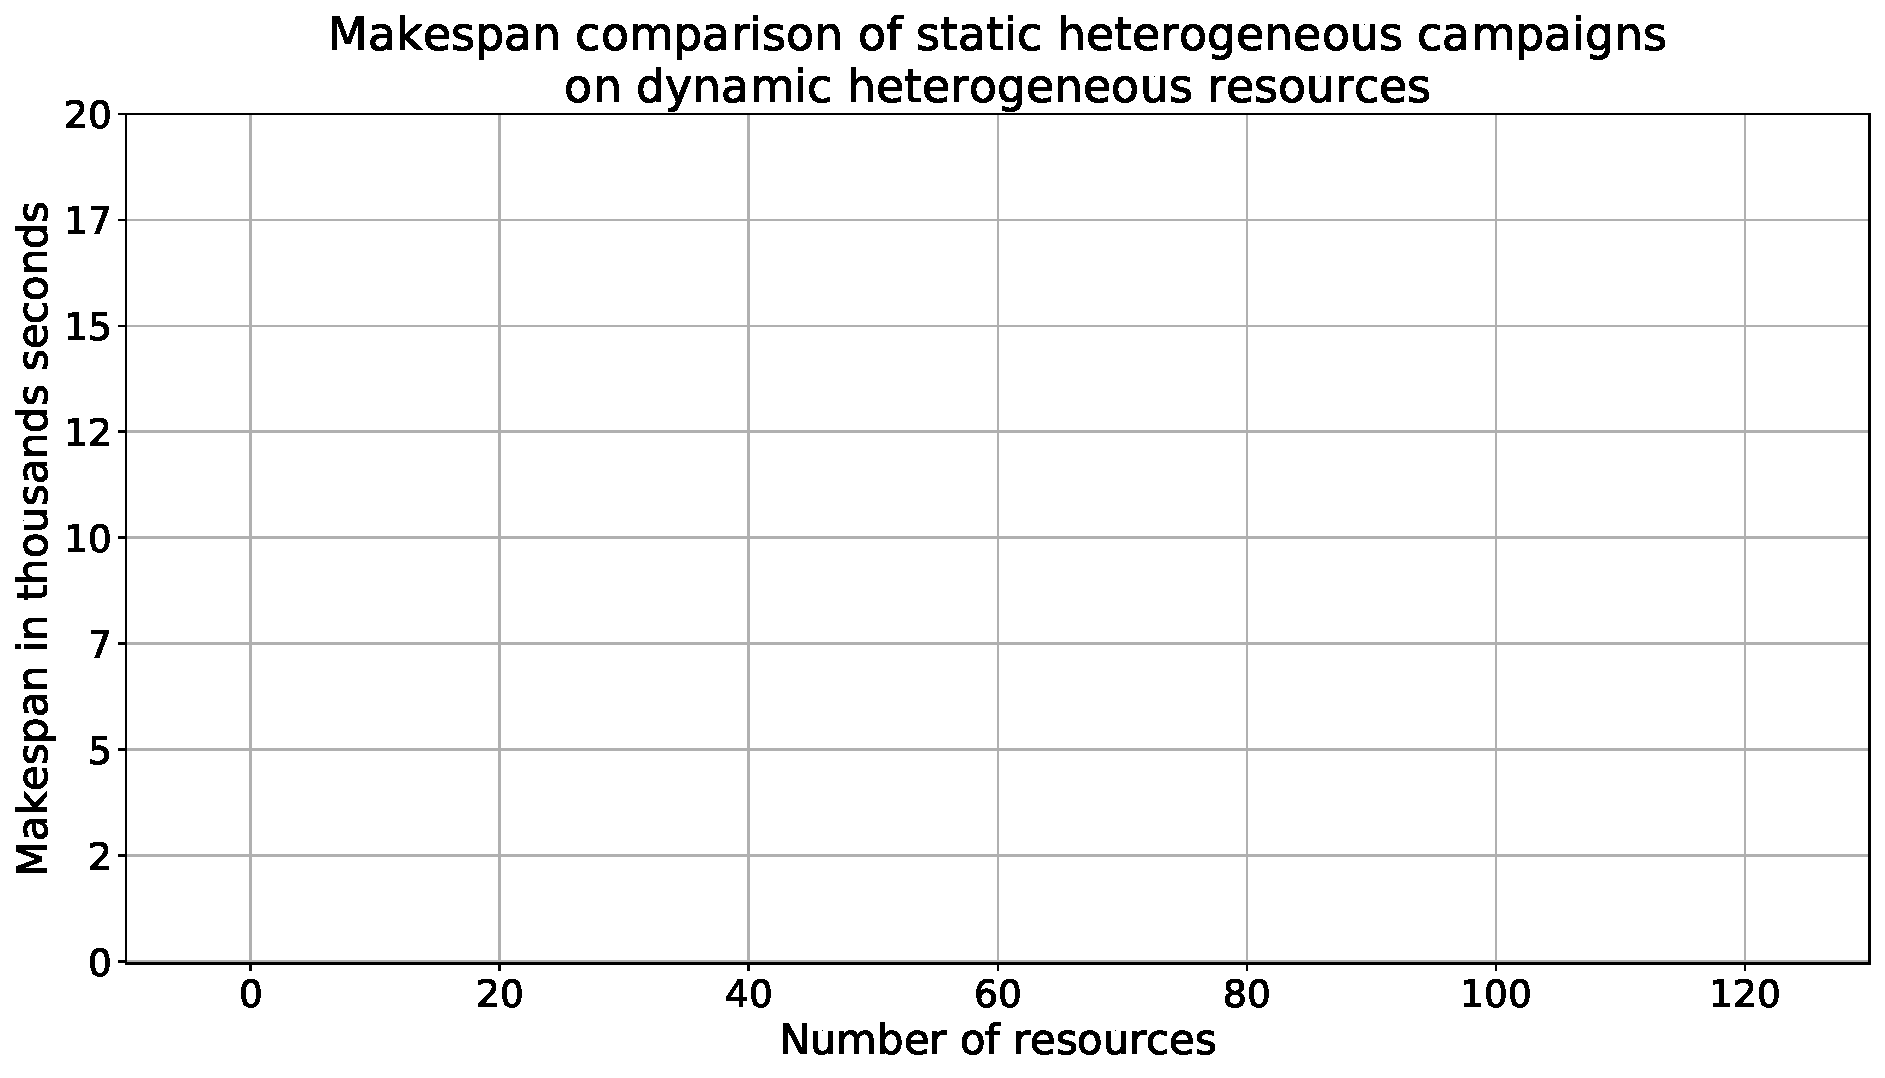
\includegraphics[width=\linewidth]{figures/campaign/DyHeteroResources_StHeteroCampaigns.pdf}
        \caption{}
        \label{fig:DyHeteroResources_StHeteroCampaignsRP}
    \end{subfigure}
    \caption{~\ref{fig:StHeteroCampaigns_4DyHeteroResourcesRP}) Makespan of increasing number of homogeneous workflows on homogeneous resources;
        ~\ref{fig:DyHeteroResources_StHeteroCampaignsRP}) Makespan of homogeneous campaign on different number of homogeneous resources.}
    \label{fig:erplan_homog_analysis}
\end{figure*}

\subsubsection{Resource availability}

Explore how HEFT and GA behave for different resource initial availability if there is time
\begin{figure*}[ht!]
    \centering
    \begin{subfigure}[b]{0.45\textwidth}
        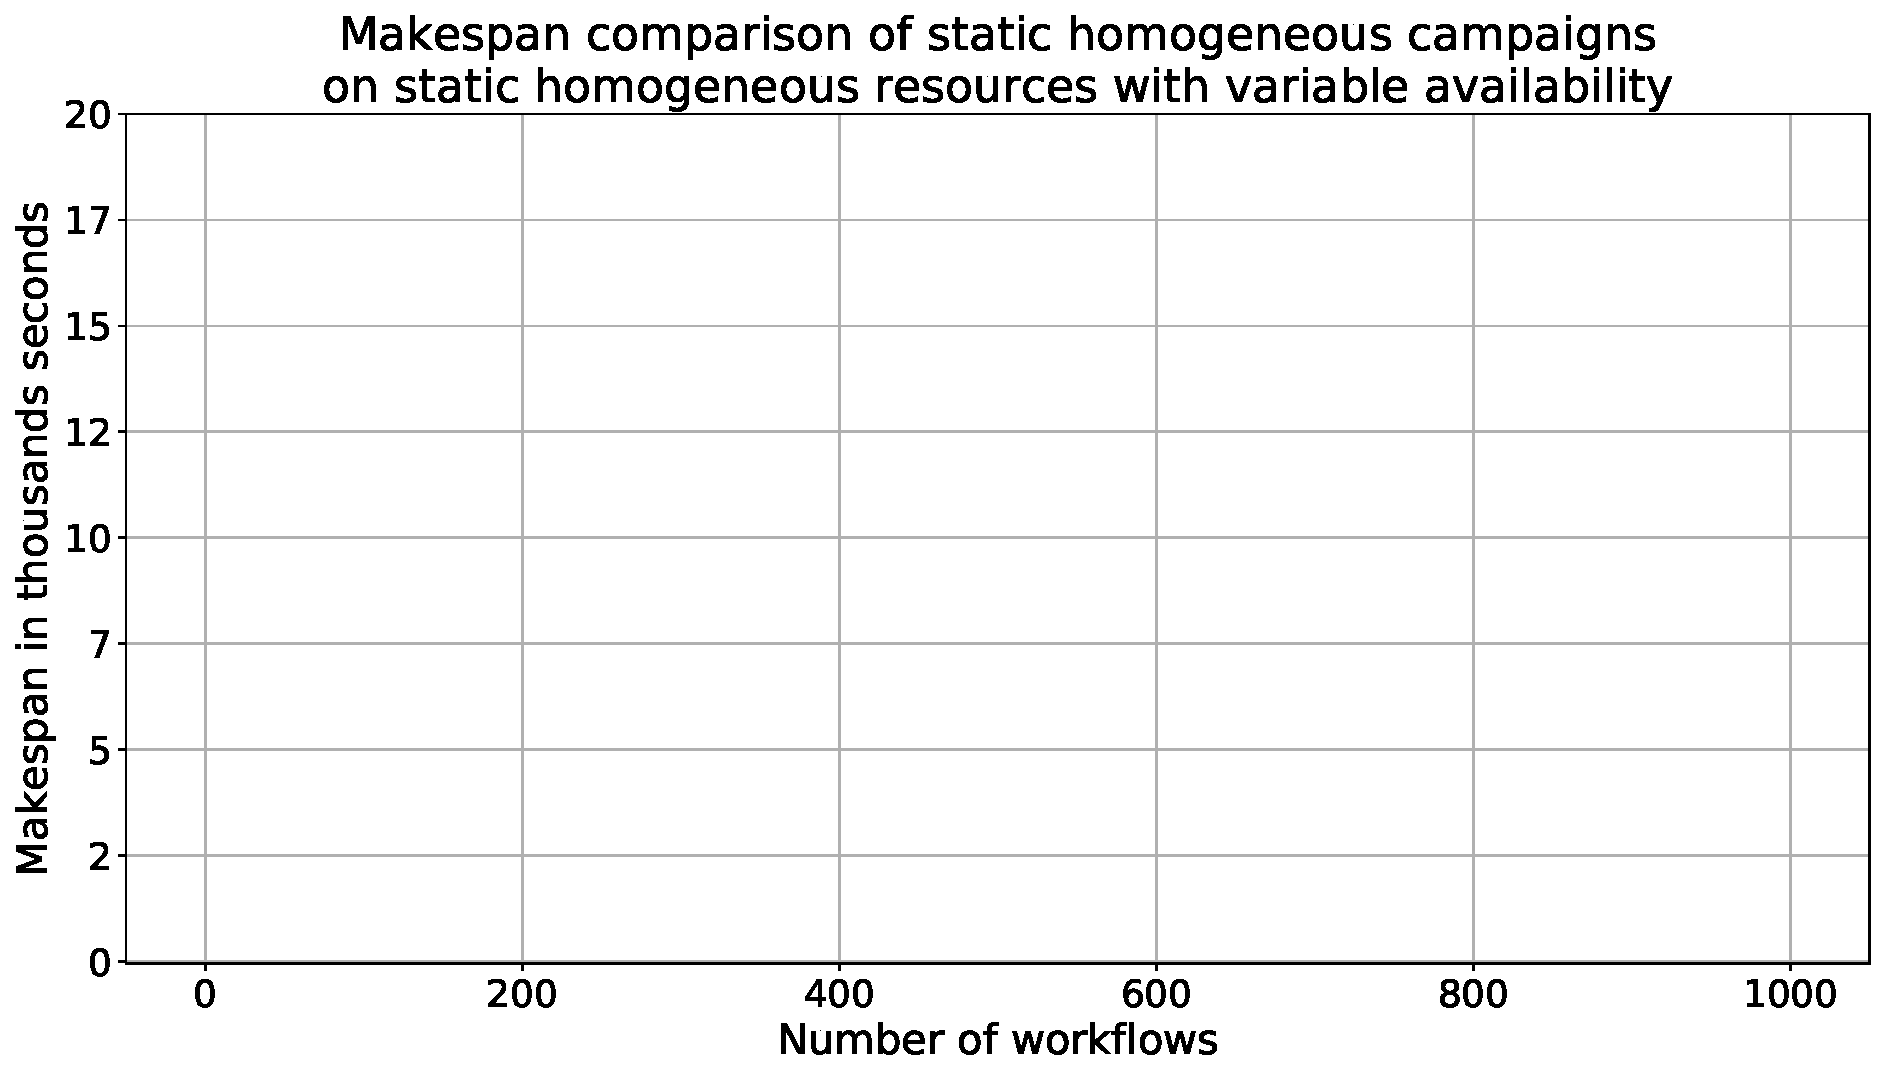
\includegraphics[width=.95\textwidth]{figures/campaign/StHomoCampaigns_4VarHomoResources.pdf}
        \caption{}
        \label{fig:StHomoCampaigns_4VarHomoResources}
    \end{subfigure}%
    ~ 
    \begin{subfigure}[b]{0.45\textwidth}
        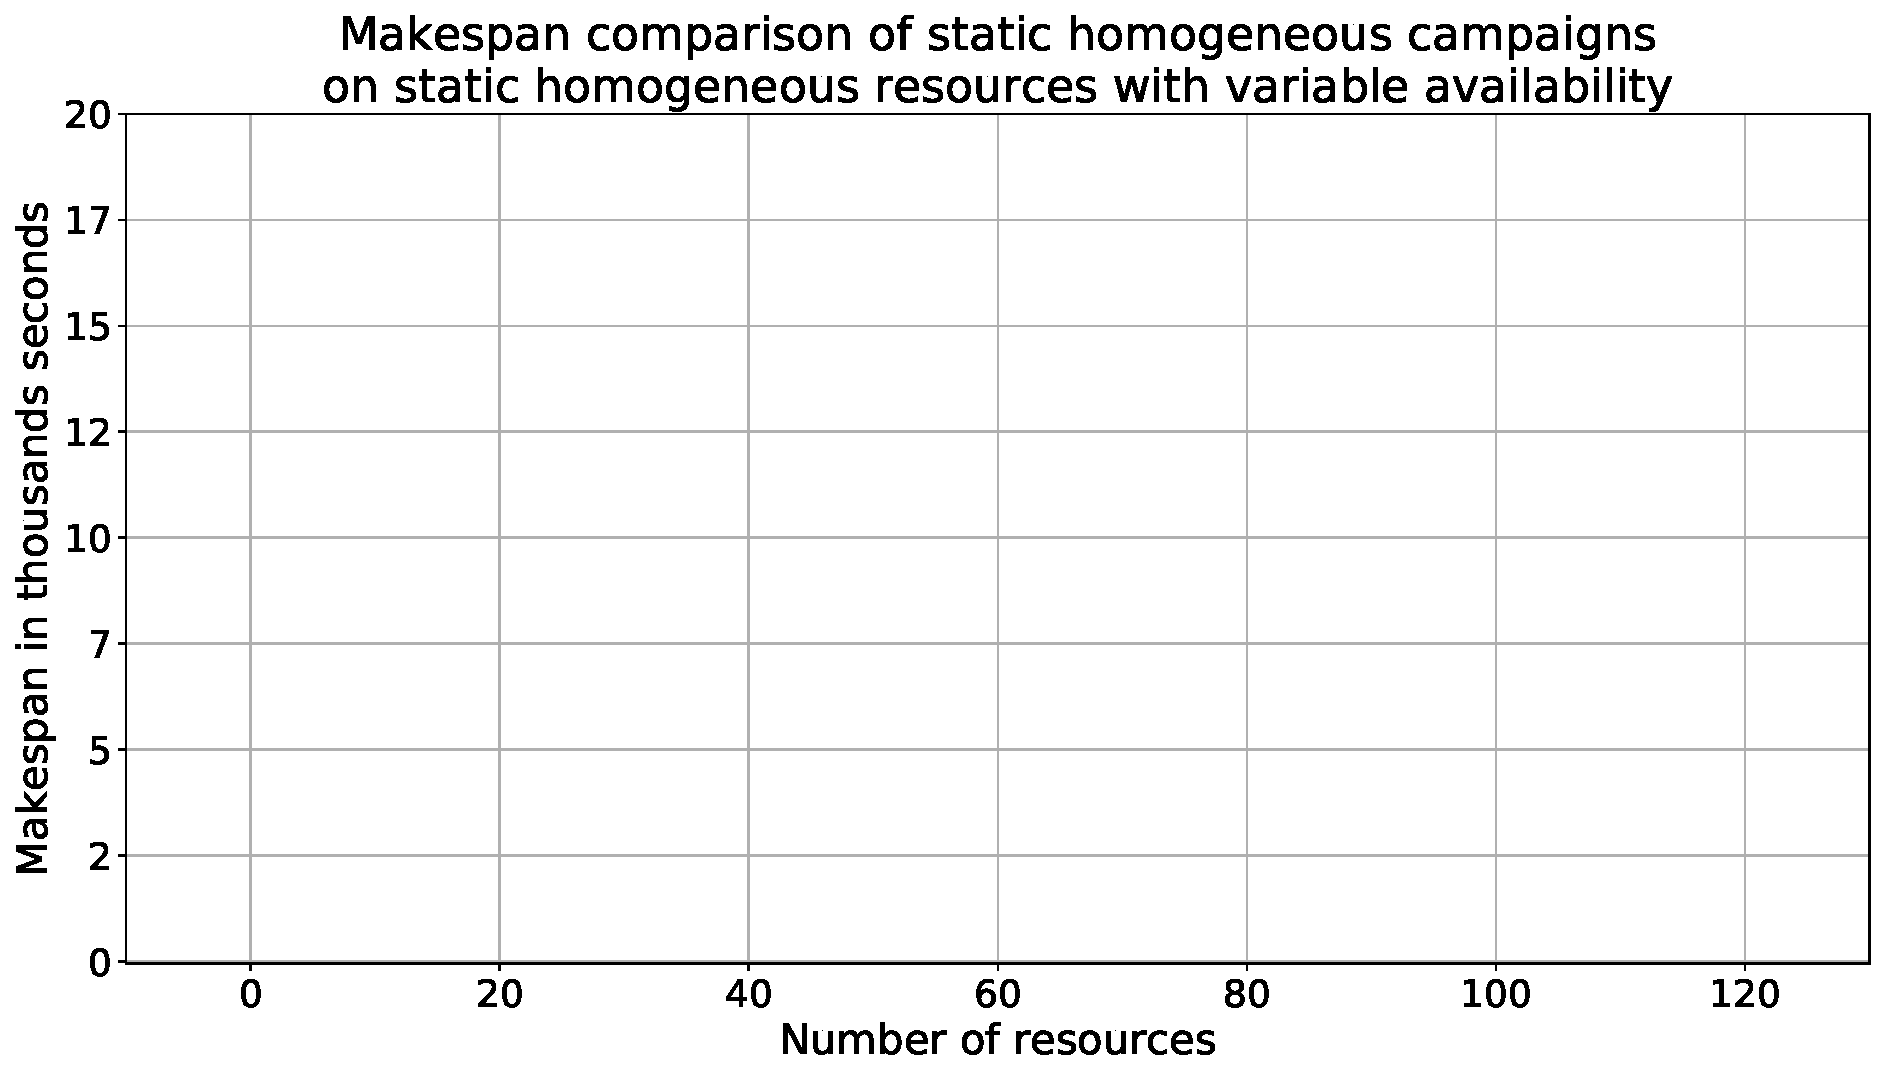
\includegraphics[width=\linewidth]{figures/campaign/VarHomoResources_StHomoCampaigns.pdf}
        \caption{}
        \label{fig:VarHomoResources_StHomoCampaigns}
    \end{subfigure}
    \caption{~\ref{fig:StHomoCampaigns_4VarHomoResources} Makespan of increasing number of homogeneous workflows on homogeneous resources;
    ~\ref{fig:VarHomoResources_StHomoCampaigns} Makespan of homogeneous campaign on different number of homogeneous resources.}
    \label{fig:resource_avail}
\end{figure*}

\subsubsection{Time to calculate a plan}

Based on experiments HEFT and L2FF will have the smallest overhead for calculating the makespan.
This is due to their deterministic behavior.
GA on the other hand is a non-deterministic algorithm and its runtime depends on its convergence rate.

\section{Conclusions}

Based on our analysis, we conclude that selecting algorithm1 over algorithm2 provides the better makespan in most cases. 
But due to the time scales at which the execution of a campaign runs, the computation complexity of the algorithm, as long as, it remains in the order of minutes is not significant.
In addition, selecting an algorithm that can encode resource availability is beneficial, since resources can become unavailable either due to performance dynamism, or due to unforeseen events